\documentclass[paper=letter,11pt]{scrartcl}

\KOMAoptions{headinclude=true, footinclude=false}
\KOMAoptions{DIV=14, BCOR=5mm}
\KOMAoptions{numbers=noendperiod}
\KOMAoptions{parskip=half}
\addtokomafont{disposition}{\rmfamily}
\addtokomafont{part}{\LARGE}
\addtokomafont{descriptionlabel}{\rmfamily}
%\setkomafont{pageheadfoot}{\normalsize\sffamily}
\setkomafont{pagehead}{\normalsize\rmfamily}
%\setkomafont{publishers}{\normalsize\rmfamily}
\setkomafont{caption}{\normalfont\small}
\setcapindent{0pt}
\deffootnote[1em]{1em}{1em}{\textsuperscript{\thefootnotemark}\ }


\usepackage{amsmath}
\usepackage[varg]{txfonts}
\usepackage[T1]{fontenc}
\usepackage{graphicx}
\usepackage{xcolor}
\usepackage[american]{babel}
% hyperref is needed in many places, so include it here
\usepackage{hyperref}

\usepackage{xspace}
\usepackage{multirow}
\usepackage{float}


\usepackage{braket}
\usepackage{bbm}
\usepackage{relsize}
\usepackage{tcolorbox}

\def\ketY{\ensuremath{\ket {\Psi}}}
\def\iGeV{\ensuremath{\textrm{GeV}^{-1}}}
%\def\mp{\ensuremath{m_{\textrm{proton}}}}
\def\rp{\ensuremath{r_{\textrm{proton}}}}
\def\me{\ensuremath{m_{\textrm{electron}}}}
\def\aG{\ensuremath{\alpha_G}}
\def\rAtom{\ensuremath{r_{\textrm{atom}}}}
\def\rNucl{\ensuremath{r_{\textrm{nucleus}}}}
\def\GN{\ensuremath{\textrm{G}_\textrm{N}}}
\def\ketX{\ensuremath{\ket{\vec{x}}}}
\def\ve{\ensuremath{\vec{\epsilon}}}


\def\ABCDMatrix{\ensuremath{\begin{pmatrix} A &  B  \\ C  & D \end{pmatrix}}}
\def\xyprime{\ensuremath{\begin{pmatrix} x' \\ y' \end{pmatrix}}}
\def\xyprimeT{\ensuremath{\begin{pmatrix} x' &  y' \end{pmatrix}}}
\def\xy{\ensuremath{\begin{pmatrix} x \\ y \end{pmatrix}}}
\def\xyT{\ensuremath{\begin{pmatrix} x & y \end{pmatrix}}}

\def\IMatrix{\ensuremath{\begin{pmatrix} 0 &  1  \\ -1  & 0 \end{pmatrix}}}
\def\IBoostMatrix{\ensuremath{\begin{pmatrix} 0 &  1  \\ 1  & 0 \end{pmatrix}}}
\def\JThree{\ensuremath{\begin{pmatrix}    0 & -i & 0  \\ i & 0  & 0 \\ 0 & 0 & 0 \end{pmatrix}}} 
\def\JTwo{\ensuremath{\begin{bmatrix}    0 & 0 & -i  \\ 0 & 0  & 0 \\ i & 0 & 0 \end{bmatrix}}}
\def\JOne{\ensuremath{\begin{bmatrix}    0 & 0 & 0  \\ 0 & 0  & -i \\ 0 & i & 0 \end{bmatrix}}}
\def\etamn{\ensuremath{\eta_{\mu\nu}}}
\def\Lmn{\ensuremath{\Lambda^\mu_\nu}}
\def\dmn{\ensuremath{\delta^\mu_\nu}}
\def\wmn{\ensuremath{\omega^\mu_\nu}}
\def\be{\begin{equation*}}
\def\ee{\end{equation*}}
\def\bea{\begin{eqnarray*}}
\def\eea{\end{eqnarray*}}
\def\bi{\begin{itemize}}
\def\ei{\end{itemize}}
\def\fmn{\ensuremath{F_{\mu\nu}}}
\def\fMN{\ensuremath{F^{\mu\nu}}}
\def\bc{\begin{center}}
\def\ec{\end{center}}
\def\nus{$\nu$s}

\def\adagger{\ensuremath{a_{p\sigma}^\dagger}}
\def\lineacross{\noindent\rule{\textwidth}{1pt}}

\newcommand{\multiline}[1] {
\begin{tabular} {|l}
#1
\end{tabular}
}

\newcommand{\multilineNoLine}[1] {
\begin{tabular} {l}
#1
\end{tabular}
}



\newcommand{\lineTwo}[2] {
\begin{tabular} {|l}
#1 \\
#2
\end{tabular}
}

\newcommand{\rmt}[1] {
\textrm{#1}
}


%
% Units
%
\def\m{\ensuremath{\rmt{m}}}
\def\GeV{\ensuremath{\rmt{GeV}}}
\def\pt{\ensuremath{p_\rmt{T}}}


\def\parity{\ensuremath{\mathcal{P}}}

\usepackage{cancel}
\usepackage{ mathrsfs }
\def\bigL{\ensuremath{\mathscr{L}}}

\usepackage{ dsfont }



\usepackage{fancyhdr}
\fancyhf{}


\lhead{\Large 33-444} % \hfill Introduction to Particle Physics \hfill Spring 2020}
\chead{\Large Introduction to Particle Physics} % \hfill Spring 2020}
\rhead{\Large Spring 2020} % \hfill Introduction to Particle Physics \hfill Spring 2020}

\begin{document}
\thispagestyle{fancy}

\begin{center}
{\huge \textbf{Lecture 31}}
\end{center}

{\fontsize{14}{16}\selectfont


\textbf{\underline{The Higgs Boson}}

After Symnmetry Breaking 

\be
\mathcal{L} \subset \frac{1}{4} g^2 W_\mu^- W^{+\mu} (v+h)^2 = \underbrace{\frac{1}{4} g^2v^2 W_\mu^- W^{+\mu}}_{\rmt{W's Mass Term}}  + \underbrace{\frac{1}{2} g^2v W_\mu^- W^{+\mu}h}_{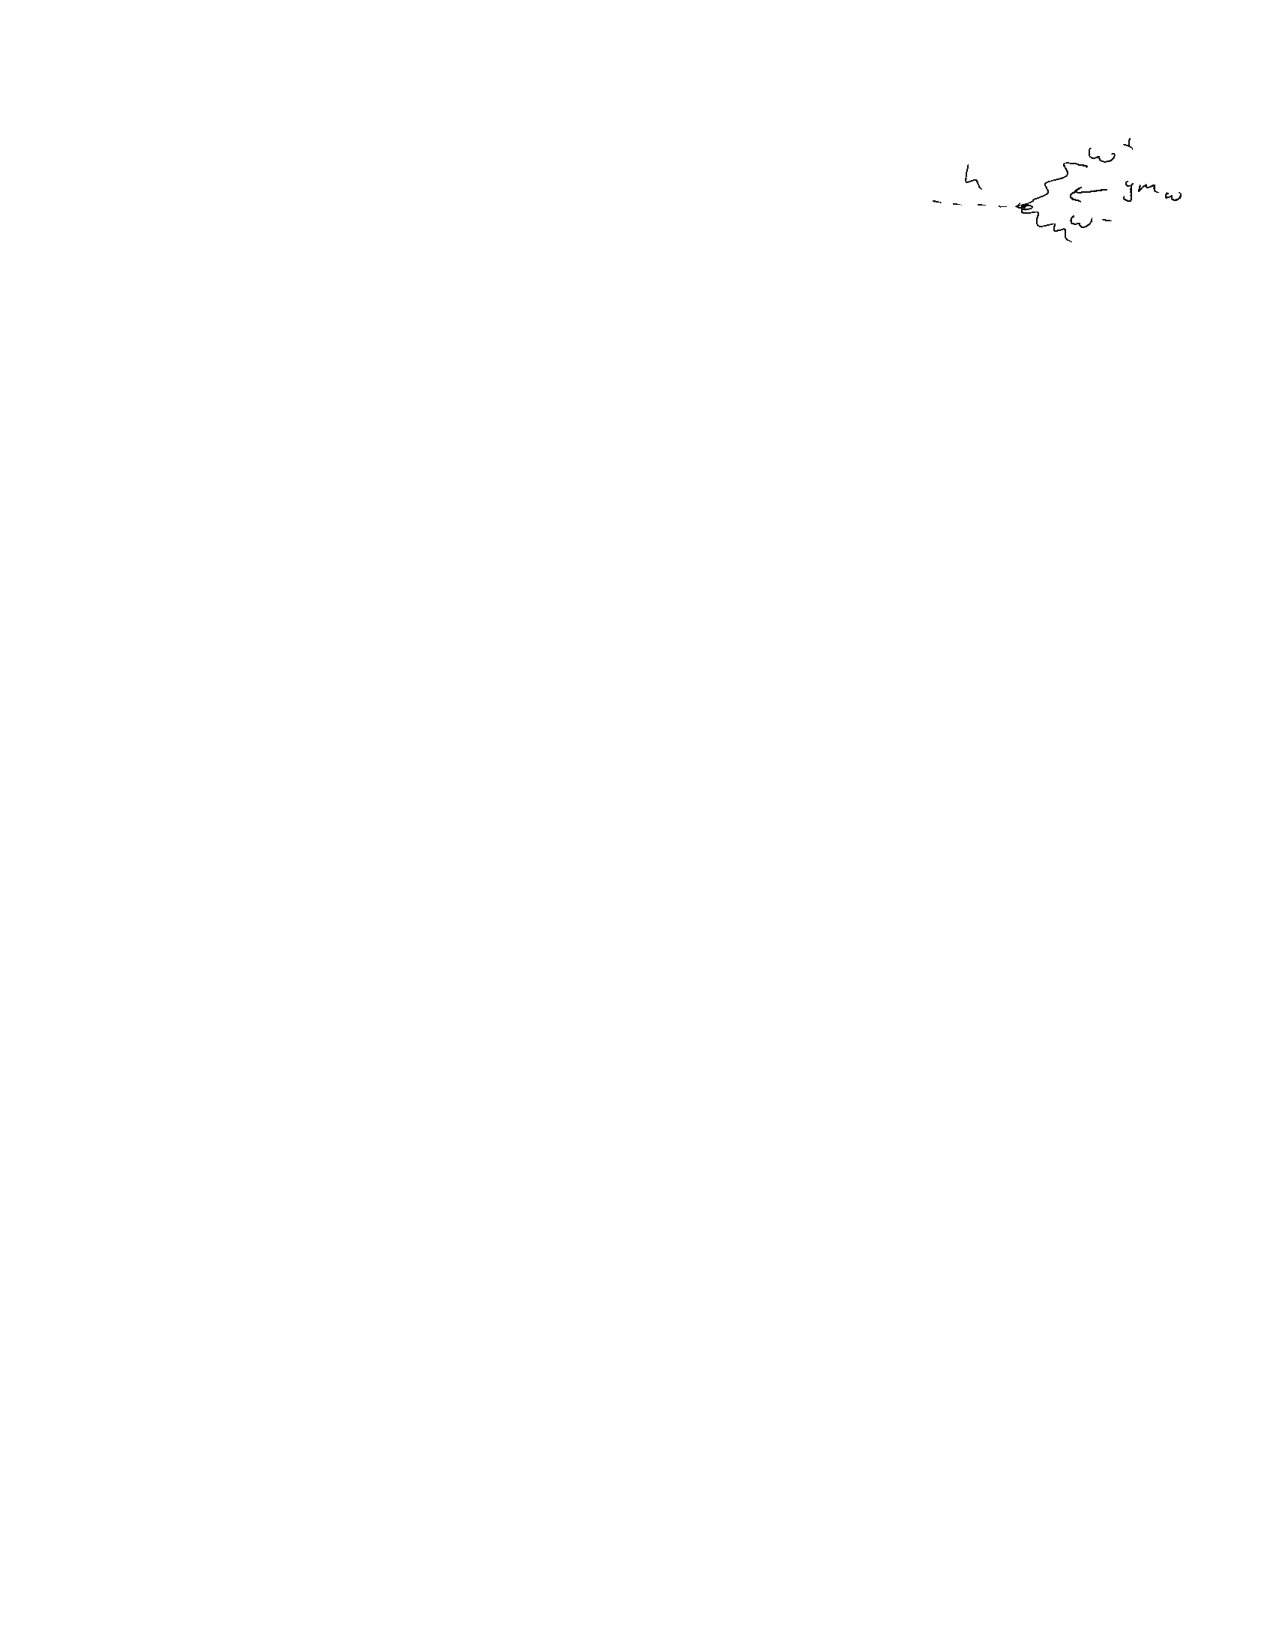
\includegraphics[width=0.25\textwidth]{./hWW.pdf}}  + \underbrace{\frac{1}{4} g^2 W_\mu^- W^{+\mu} hh}_{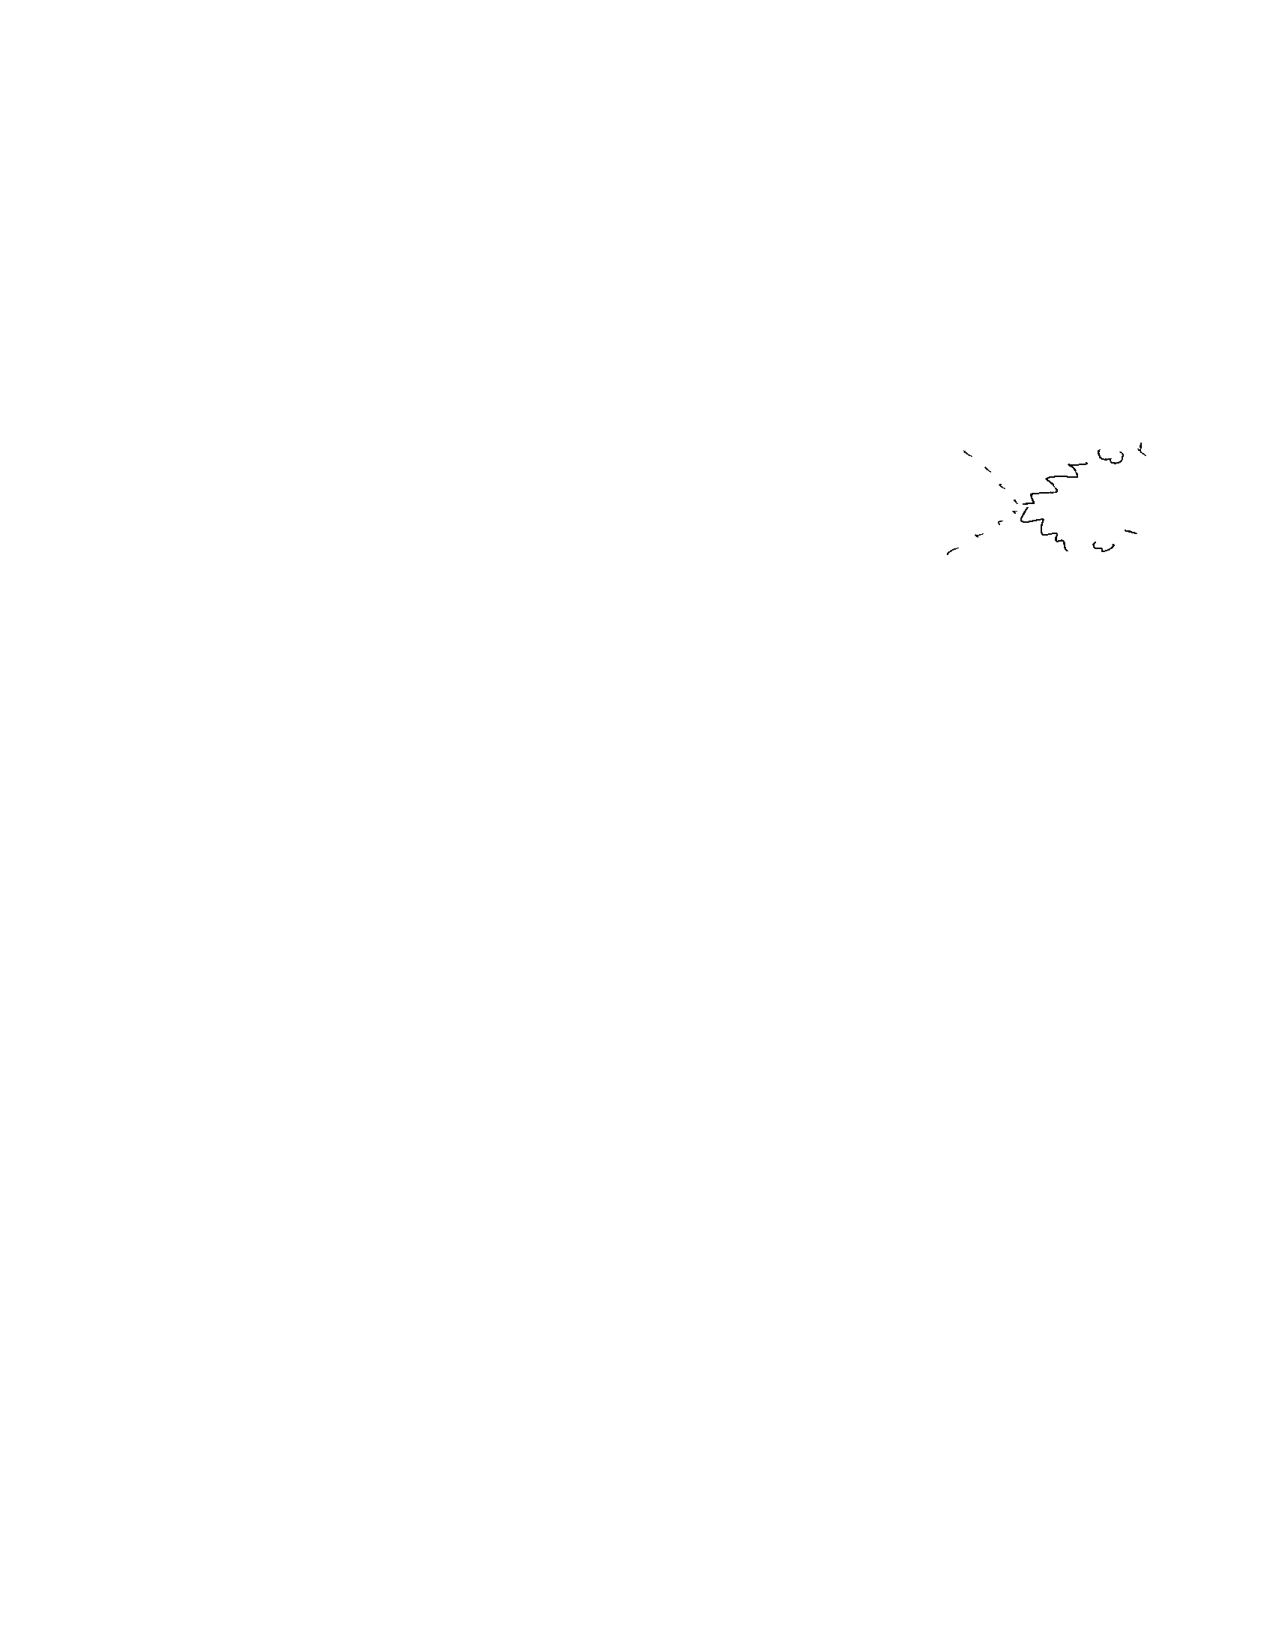
\includegraphics[width=0.25\textwidth]{./hhWW.pdf}}
\ee

Same for the Z
\bc
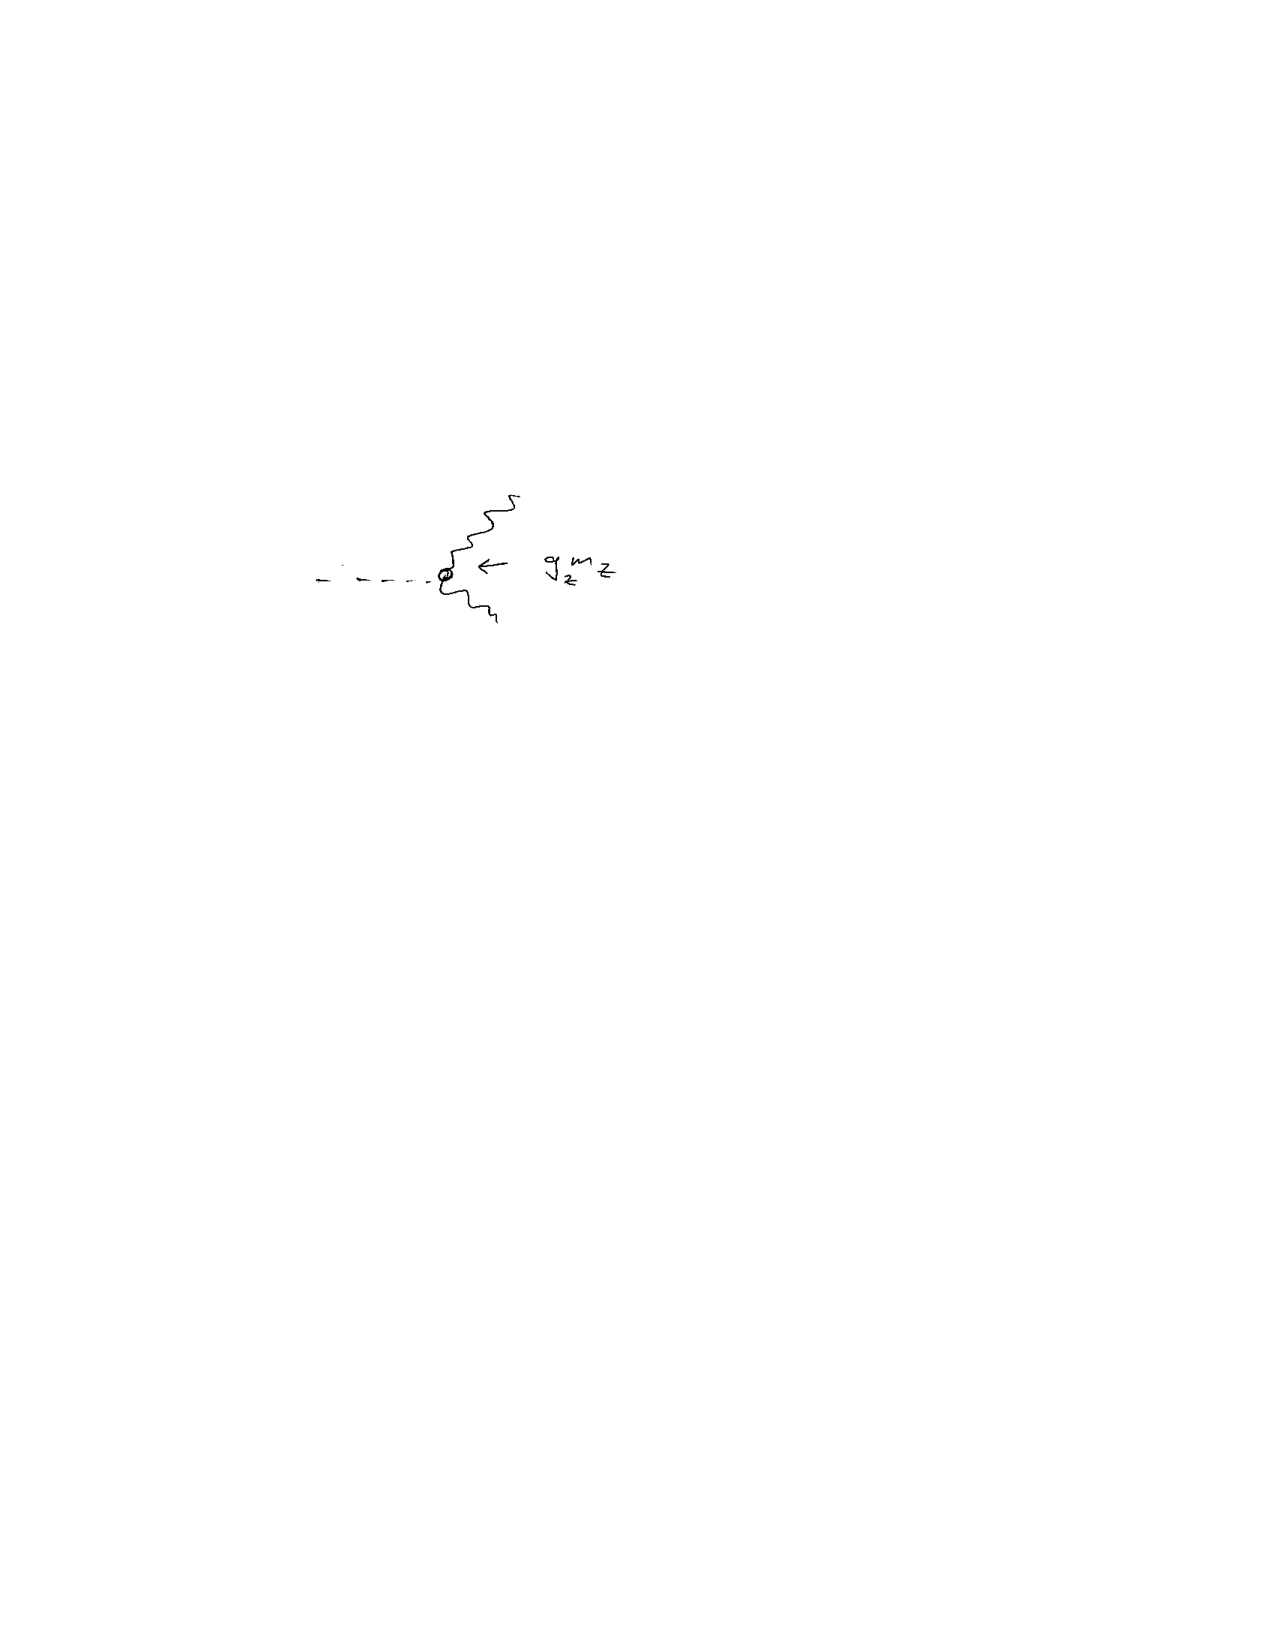
\includegraphics[width=0.5\textwidth]{./hZZ.pdf}
\ec

Saw last time Yukawa coupling leads to interactions with Higgs
\bc
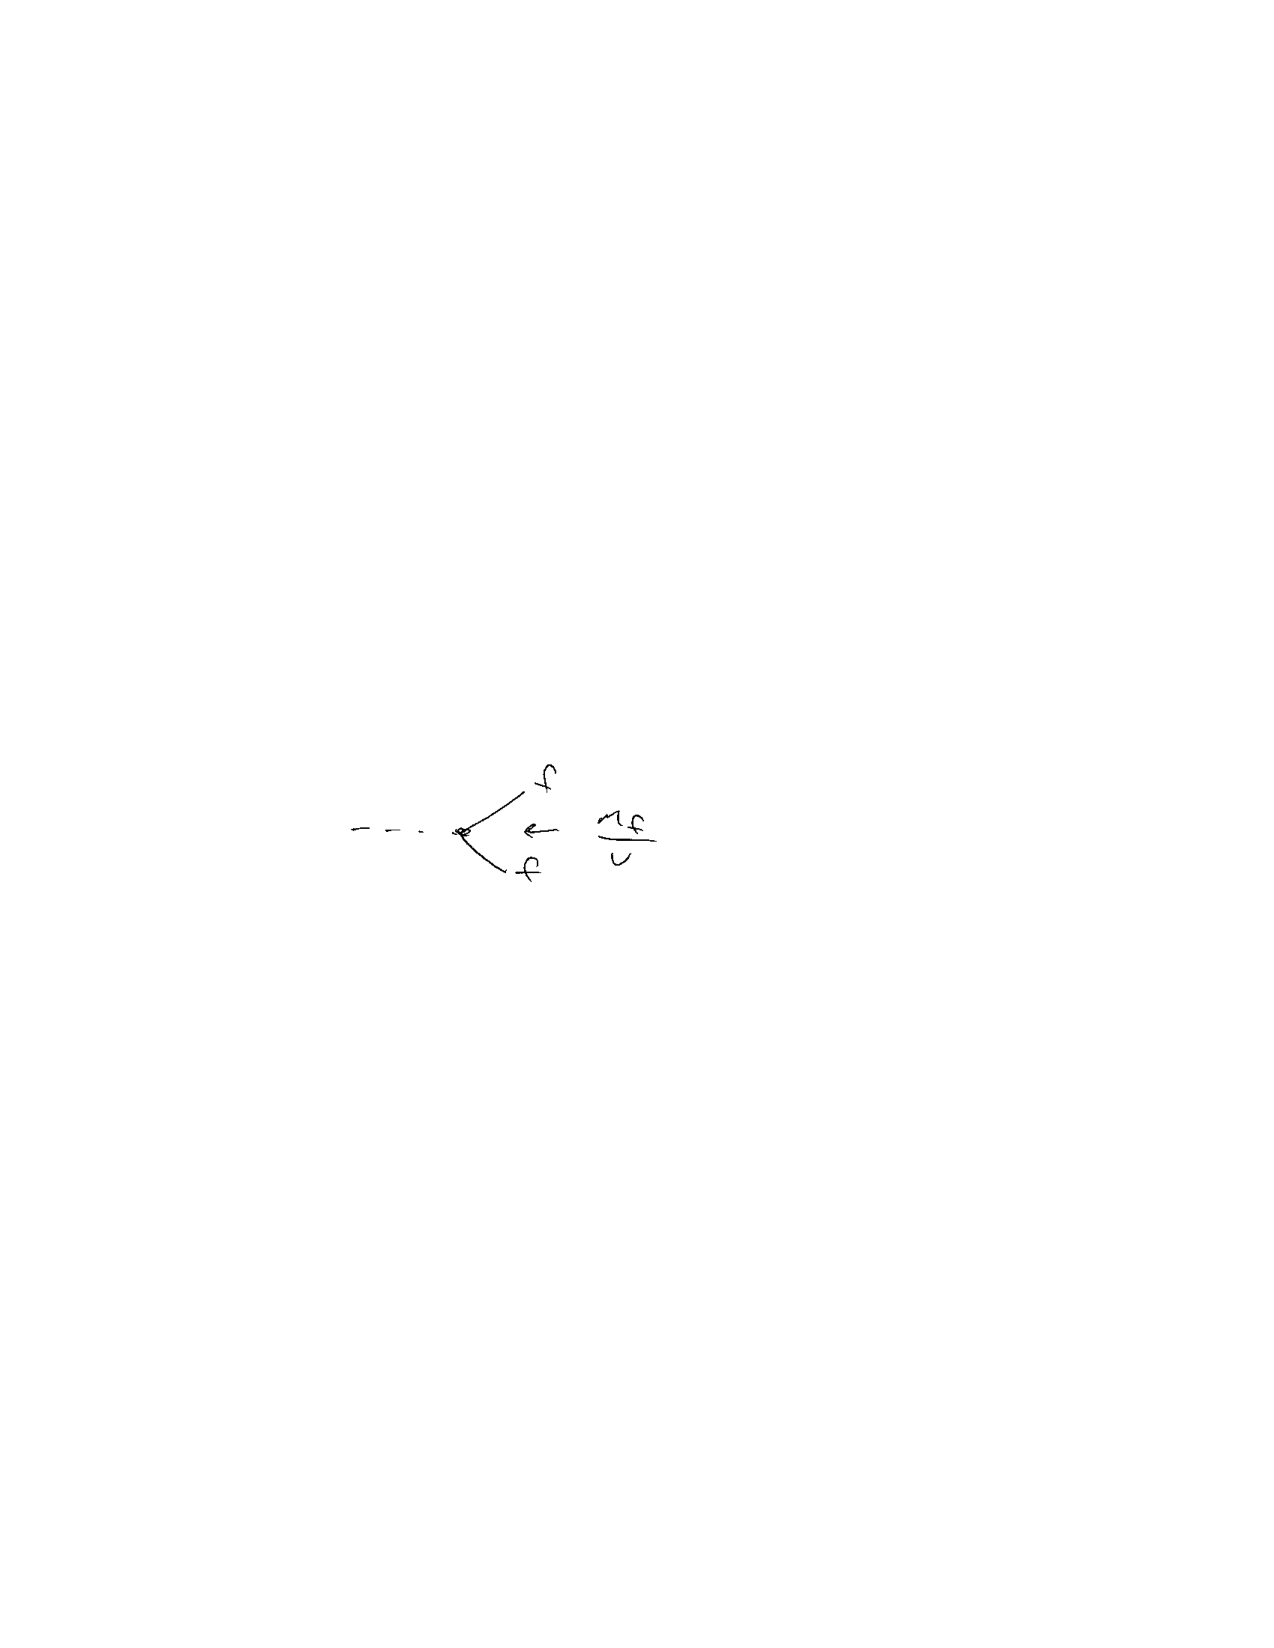
\includegraphics[width=0.5\textwidth]{./hFF.pdf}
\ec

Higgs Boson in SM is a massive neutral \underline{Spin = 0} particle. 
Its mass is free parameter ($m_H = 2\lambda v^2$)

\underline{H decays}
\bea
H &\rightarrow& ff \hspace*{1in} \rmt{if $m_H > 2m_f$}\\
H &\rightarrow& WW, ZZ \hspace*{1in} \rmt{if Massive enough}
\eea

Now, because the Higgs couples according ot mass, the Higgs wants to decay to the most massive thing it can.\\

\underline{For 125 \GeV}
\bi
\item[] Br$(h\rightarrow bb) \sim 60\%$
\item[] Br$(h\rightarrow WW) \sim 20\%$
\item[] Br$(h\rightarrow gg) \sim 10\%$
\item[] Br$(h\rightarrow \tau\tau) \sim 6\%$
\item[] Br$(h\rightarrow ZZ) \sim 3\%$
\item[] Br$(h\rightarrow \gamma\gamma) \sim 0.2\%$
\ei

\lineacross

Decays to massless particles
\bc
\includegraphics[width=0.45\textwidth]{./hgg.pdf}
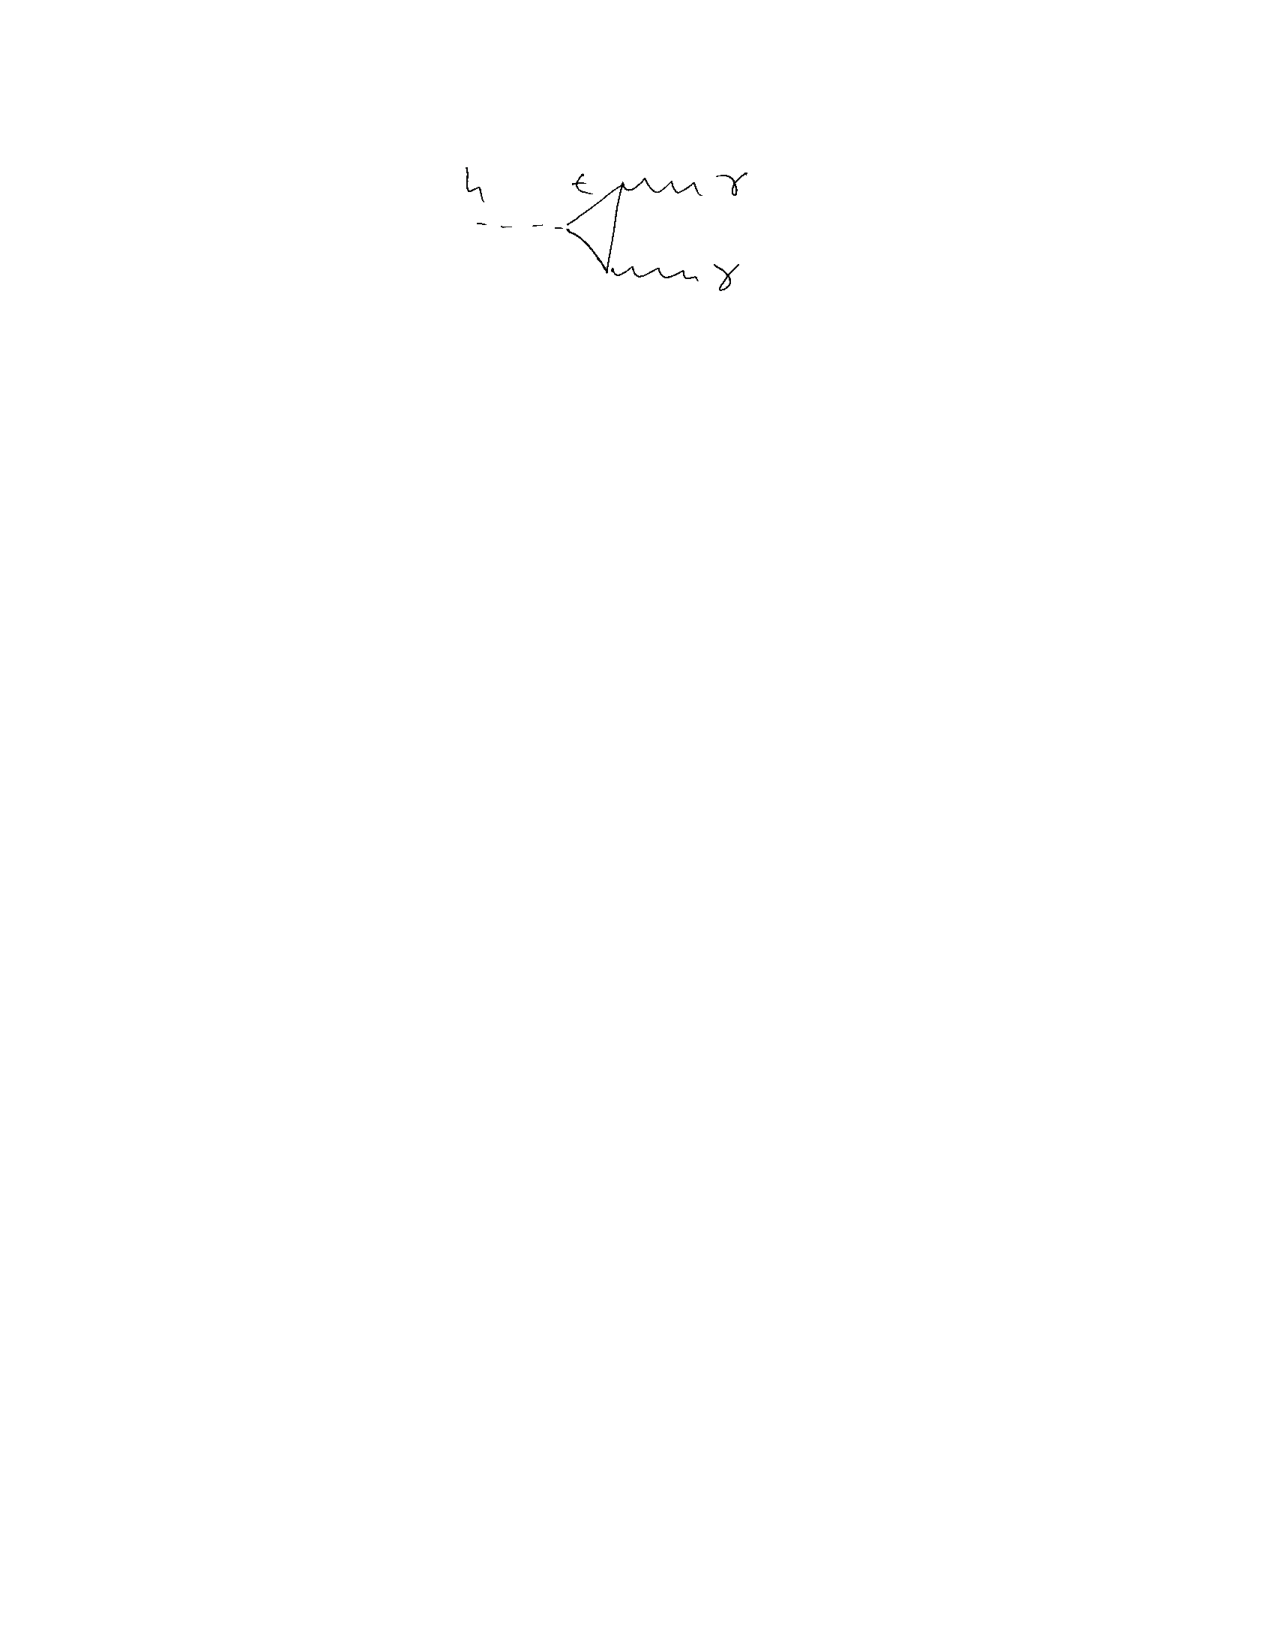
\includegraphics[width=0.45\textwidth]{./hGamGam.pdf}
\ec

Prior to LHC searched directly for the Higgs at LEP $\Rightarrow m_h > 115 \GeV$
\bc
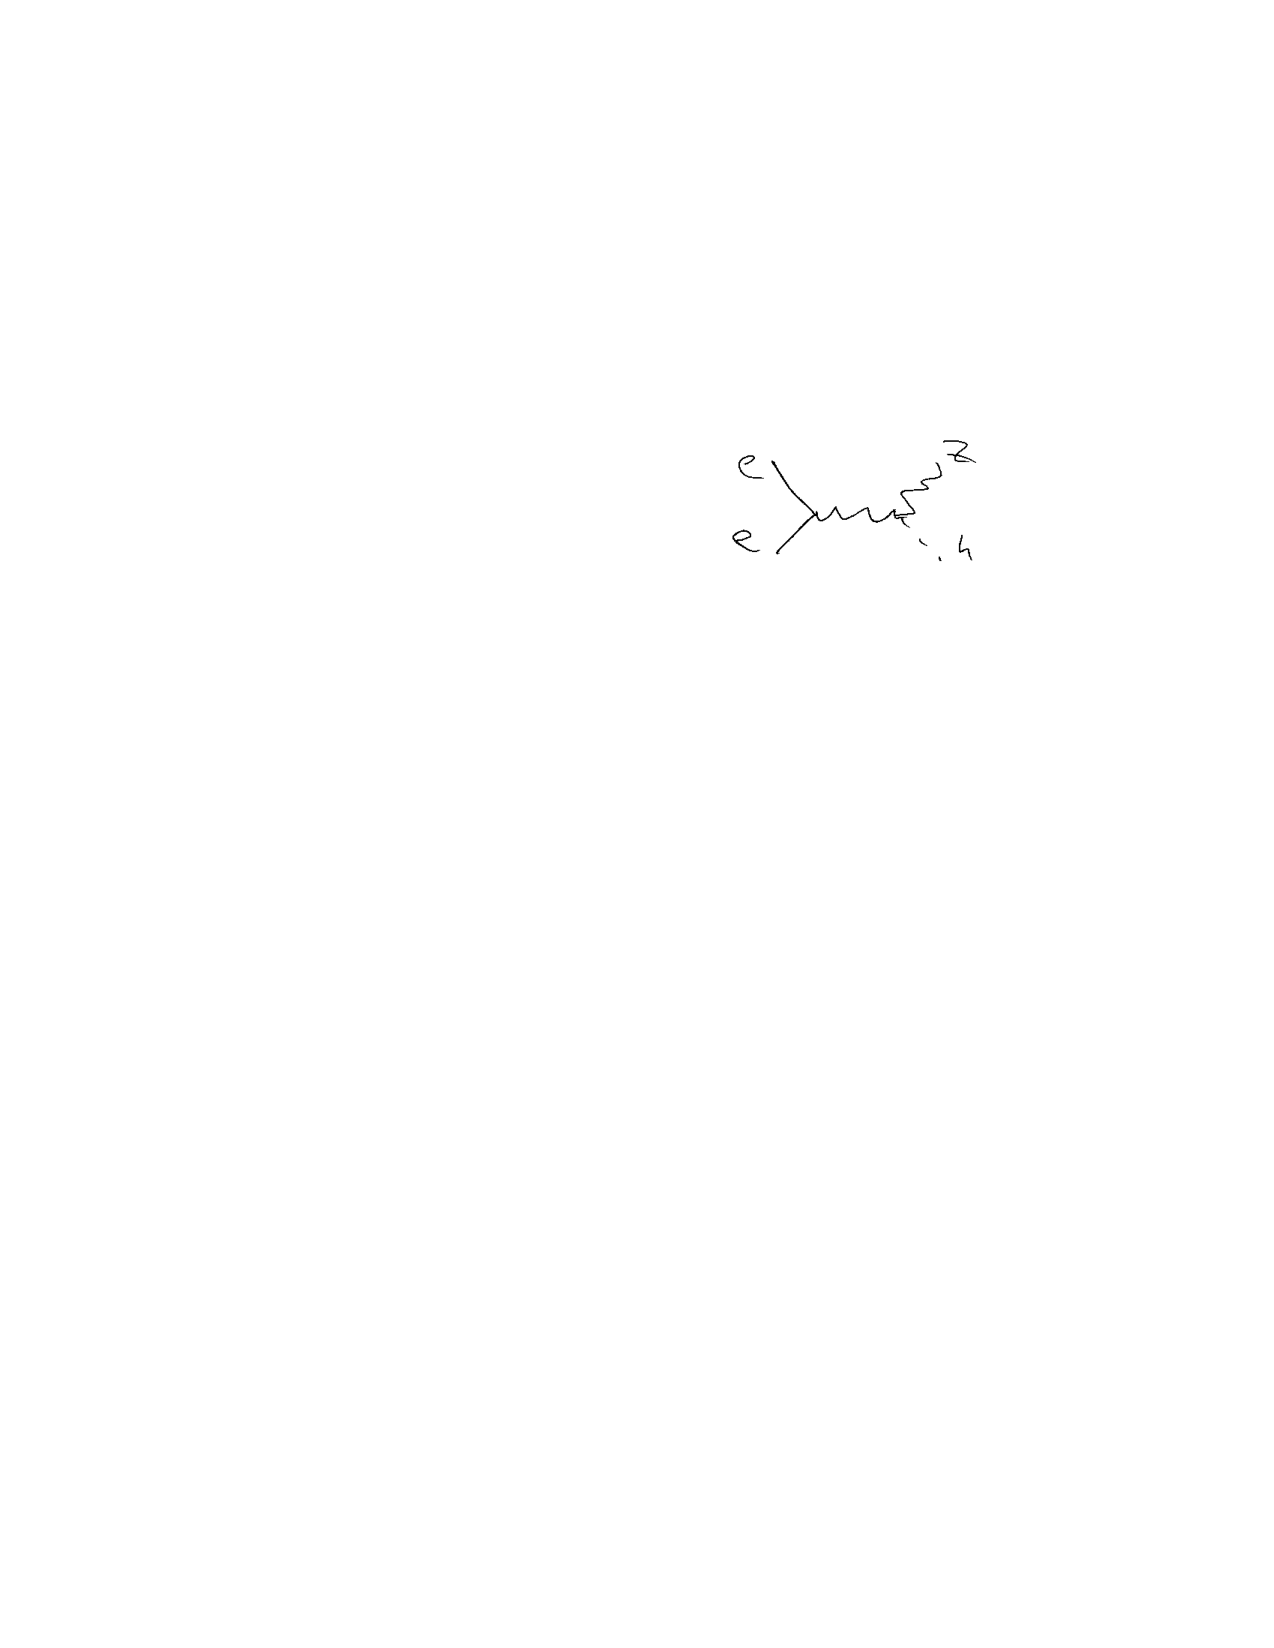
\includegraphics[width=0.3\textwidth]{./eeZH.pdf}
\ec

Also studied $m_{\rmt{top}}$ and $m_W$ which put a limit on size of $m_h$.
\bc
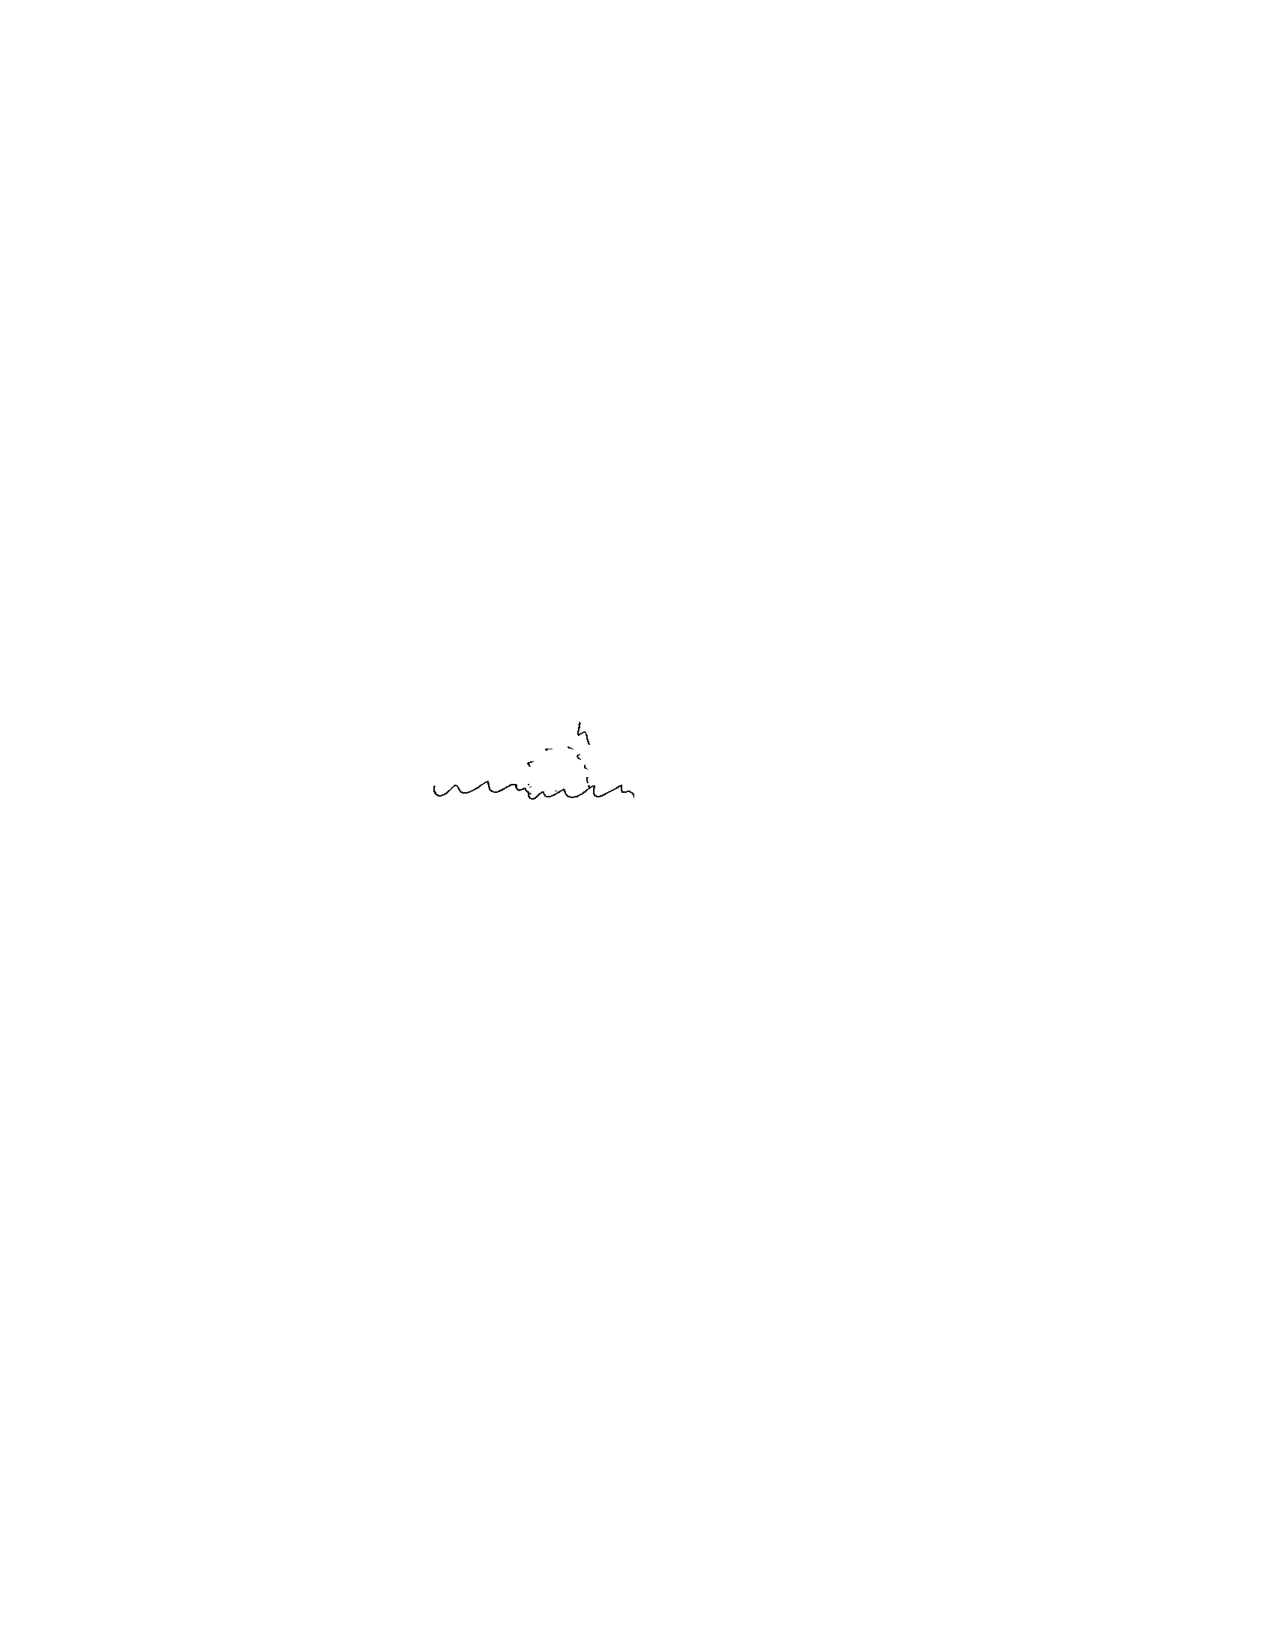
\includegraphics[width=0.4\textwidth]{./wHLoop.pdf}
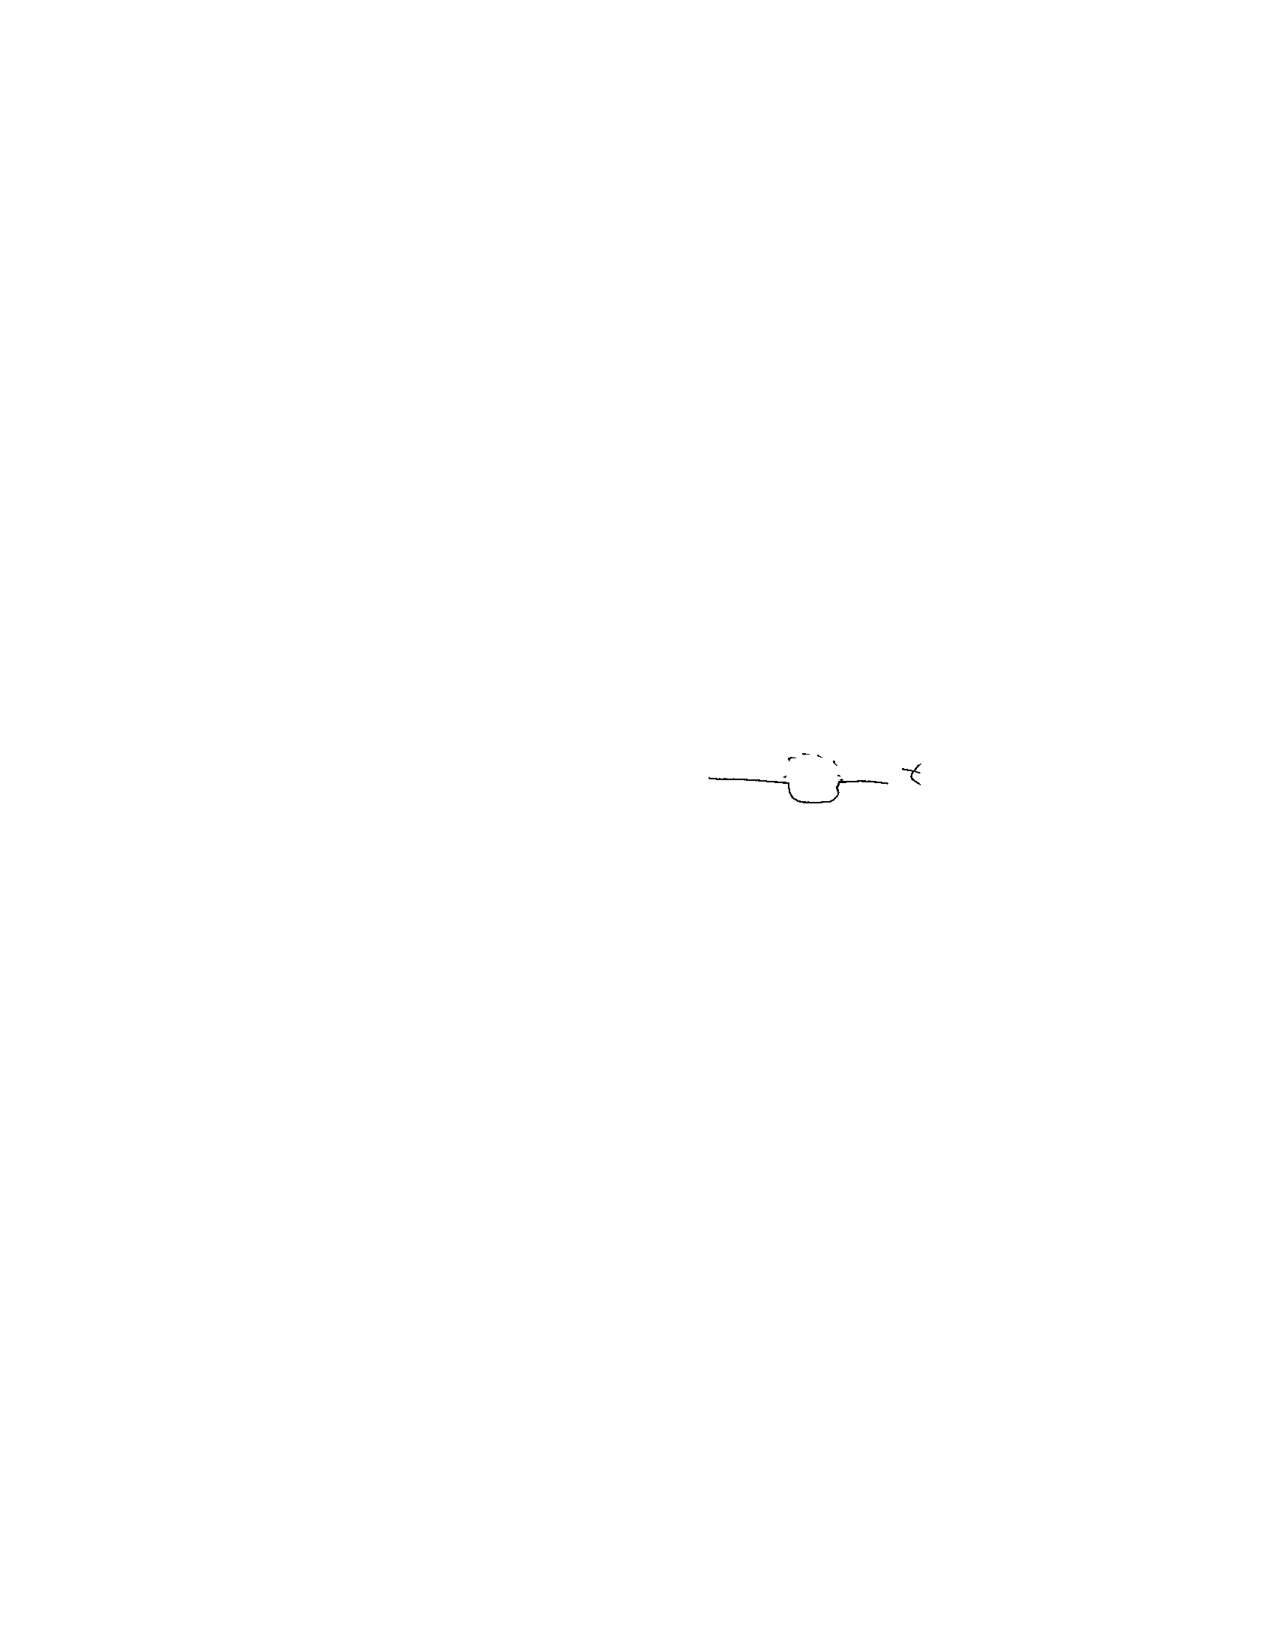
\includegraphics[width=0.4\textwidth]{./topHLoop.pdf}
\ec
$\Rightarrow m_h < 150\ \GeV$

\lineacross

Now, Major goal of LHC was to discover Higgs. 

How to make Higgs Bosons at the LHC? 

The LHC collides protons (quarks/gluons). 

\textbf{The stuff in the proton is light:}
\bi
\item[$\Rightarrow$] small coupling to the Higgs
\item[$\Rightarrow$] small cross section to produce the Higgs
\ei

top, W, and Z are the heaviest particles in the theory
$\Rightarrow$  they have the largest coupling to the higgs

Would really like to use processes like:
\bc
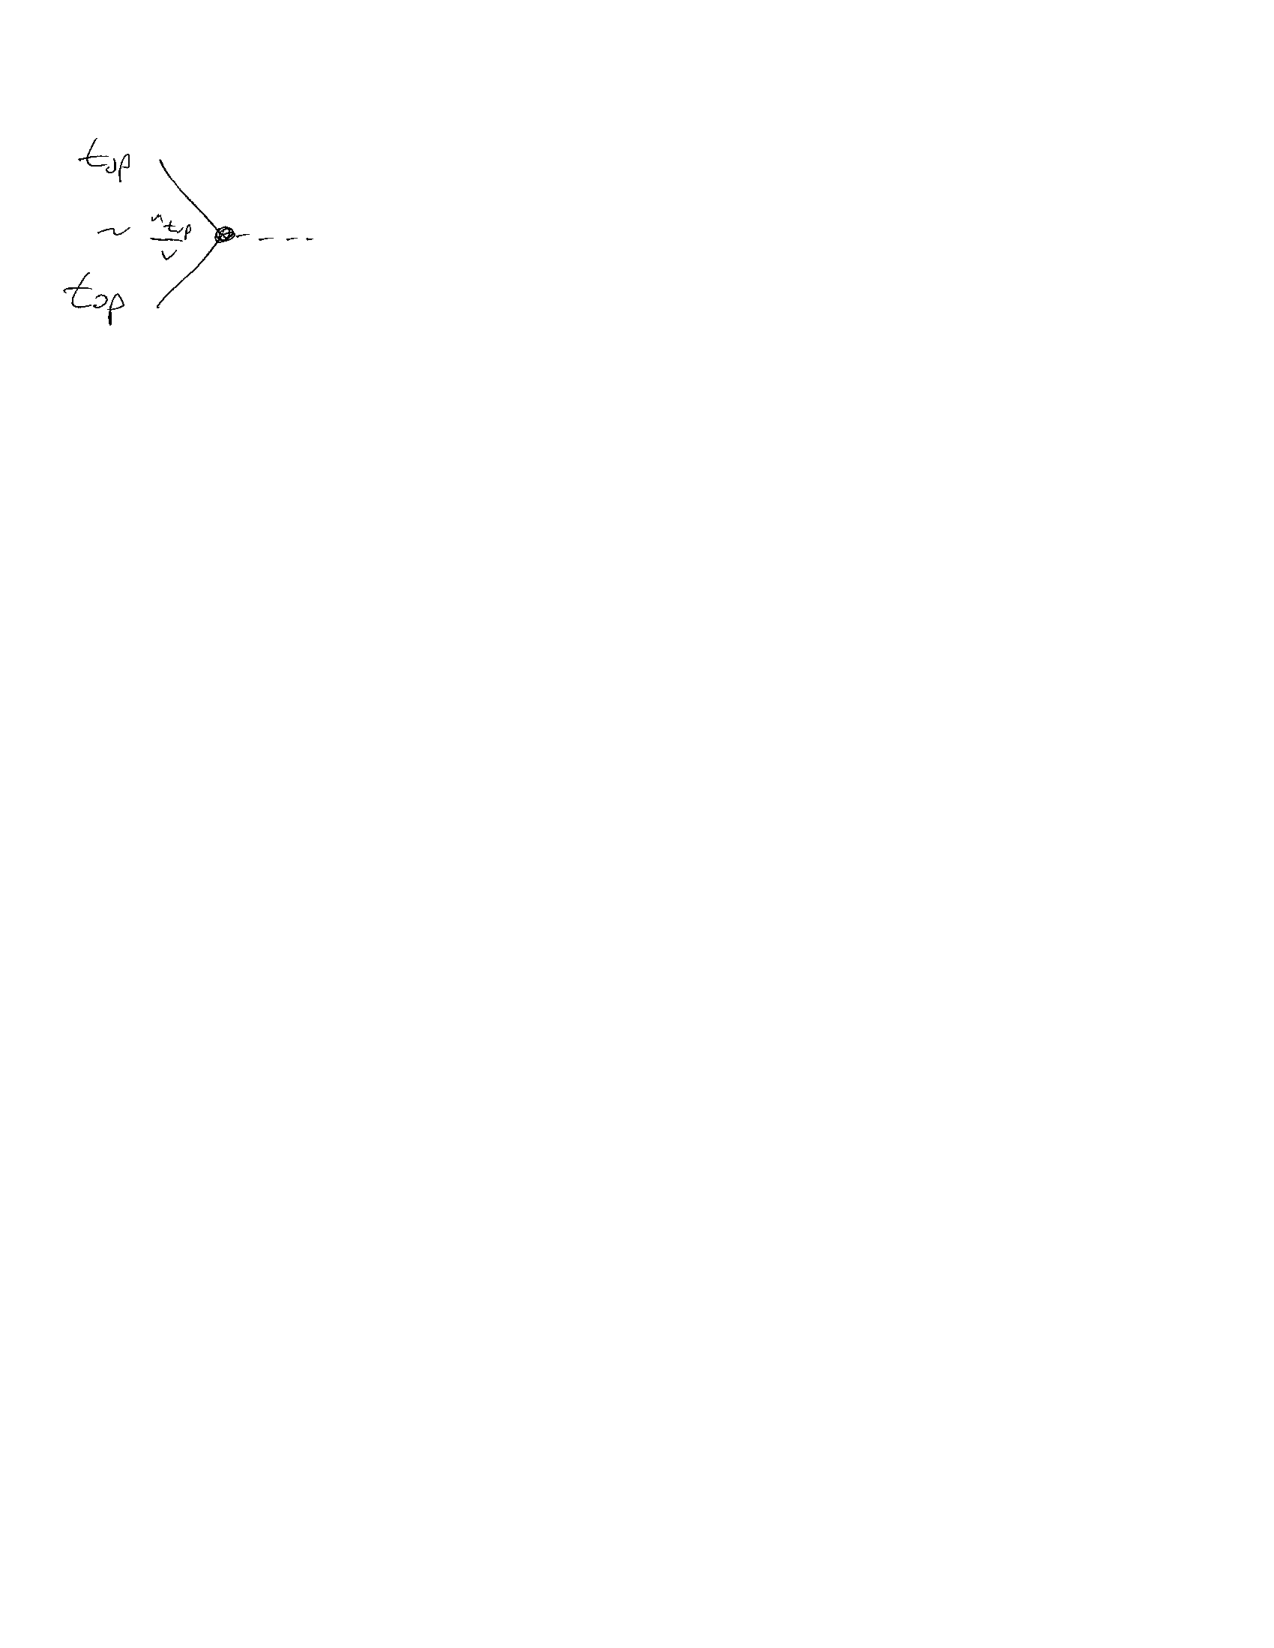
\includegraphics[width=0.3\textwidth]{./ttH.pdf}
\hspace*{0.5in}
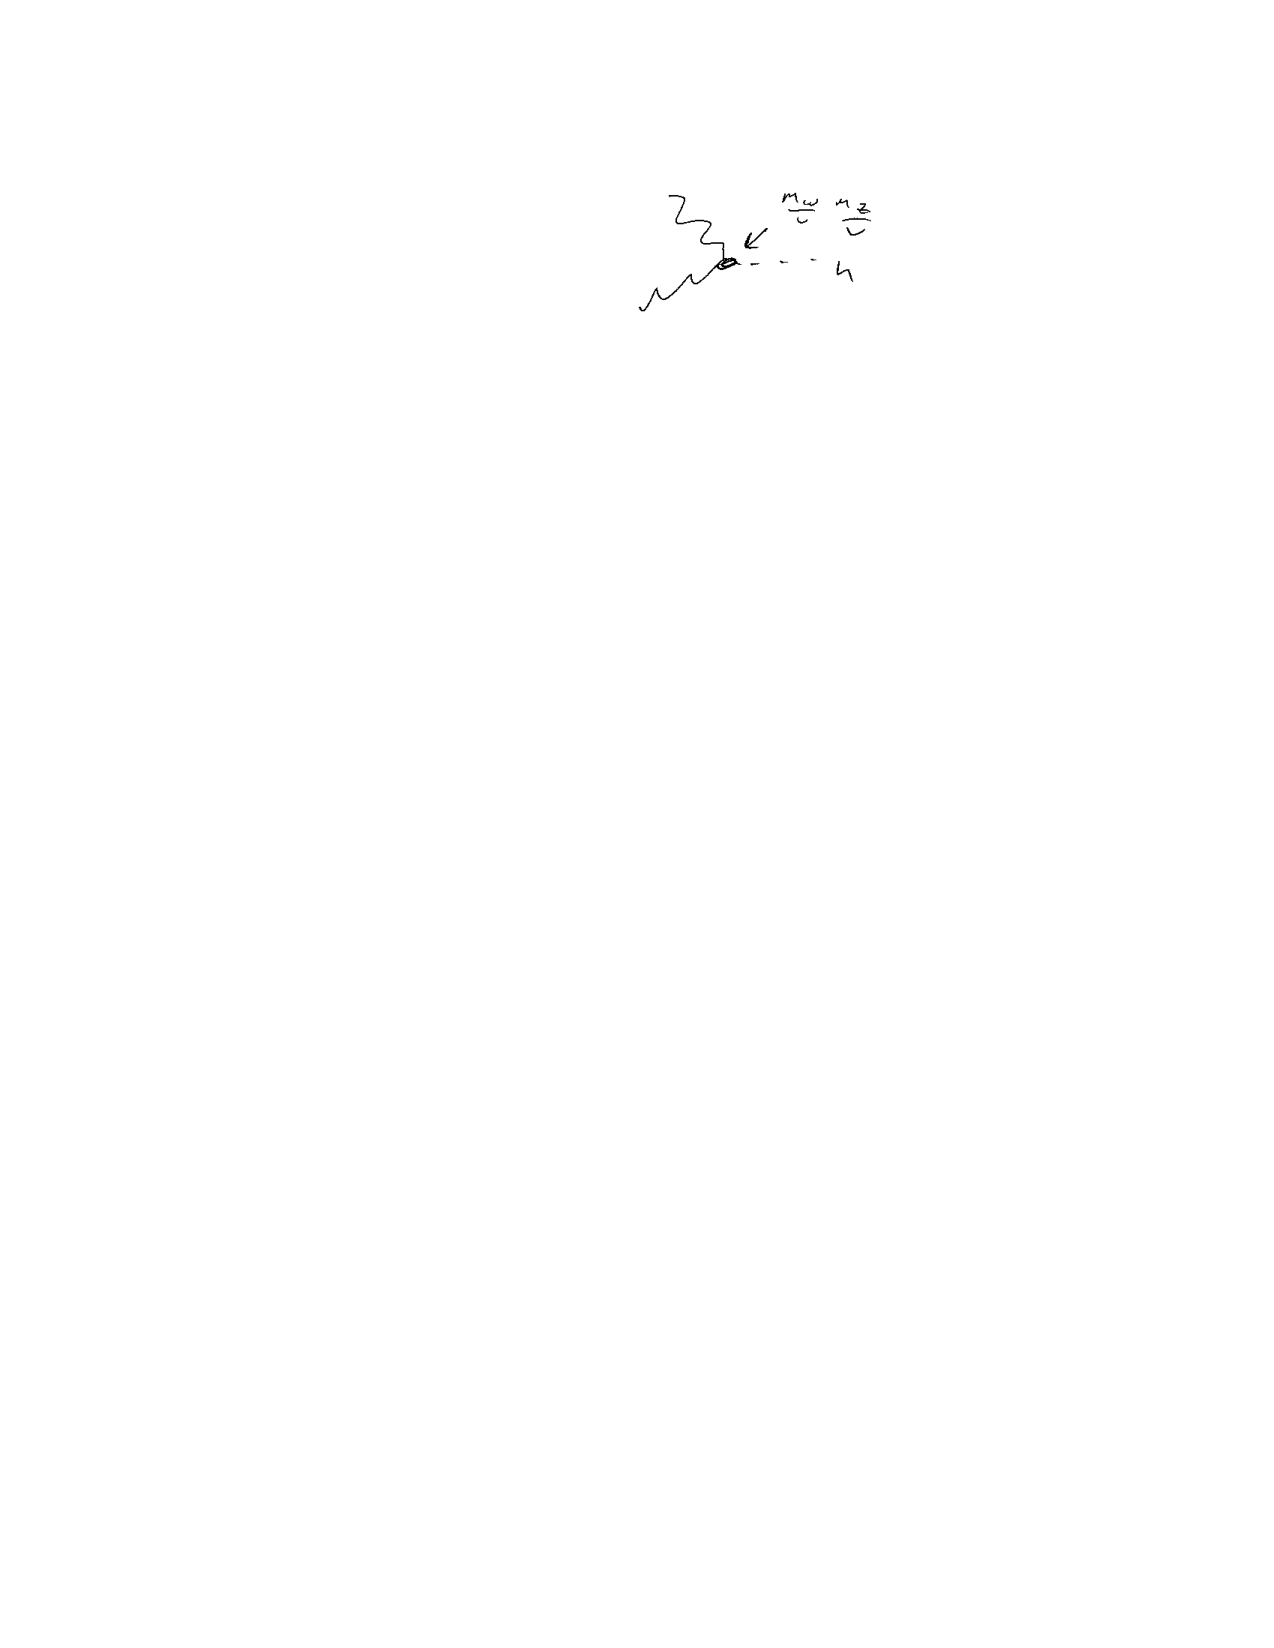
\includegraphics[width=0.3\textwidth]{./VVH.pdf}
\ec
Problem is we dont have a top/W/Z colliders.

So, at the LHC we first have to make ts Ws and Zs from protons, then make the Higgs boson.
eg: 
\be
\underbrace{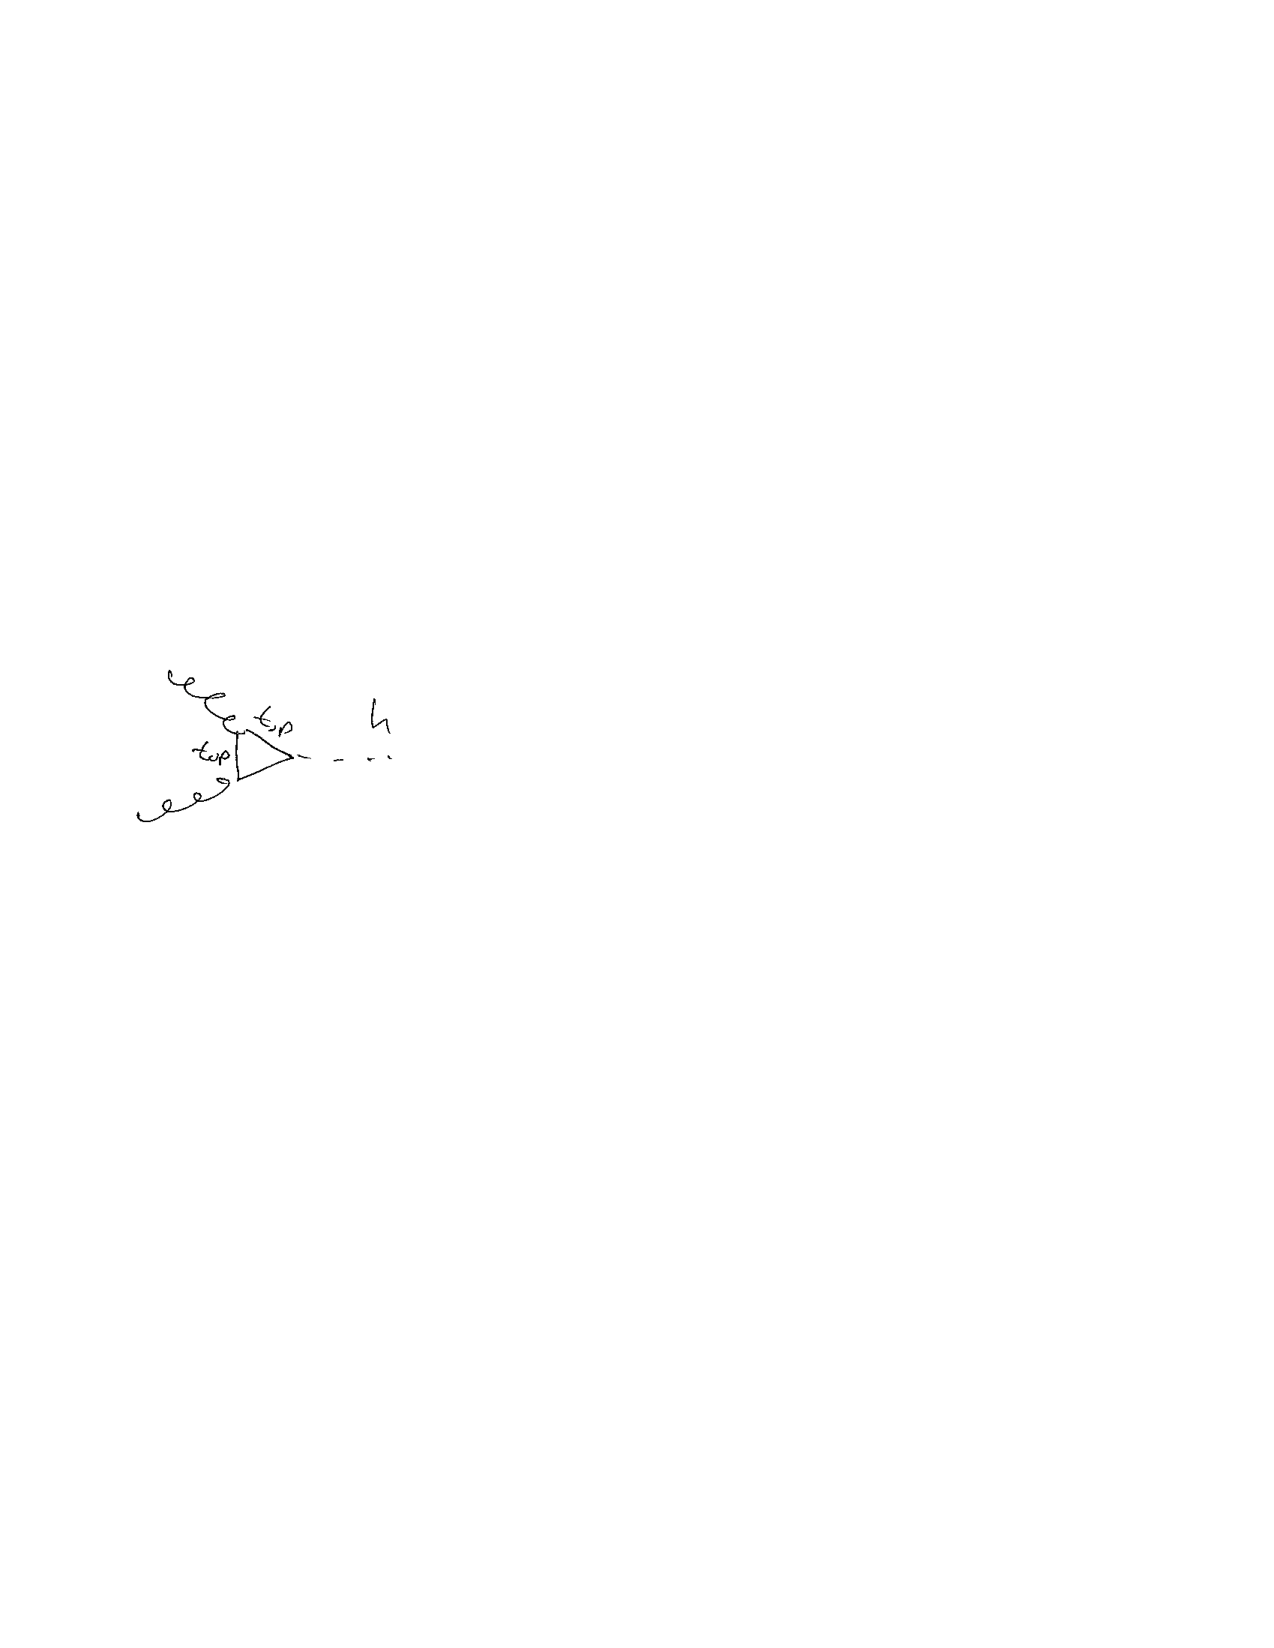
\includegraphics[width=0.4\textwidth]{./ggF.pdf}}_{\rmt{\huge ``gluon fusion''}}
\hspace*{0.2in}
\underbrace{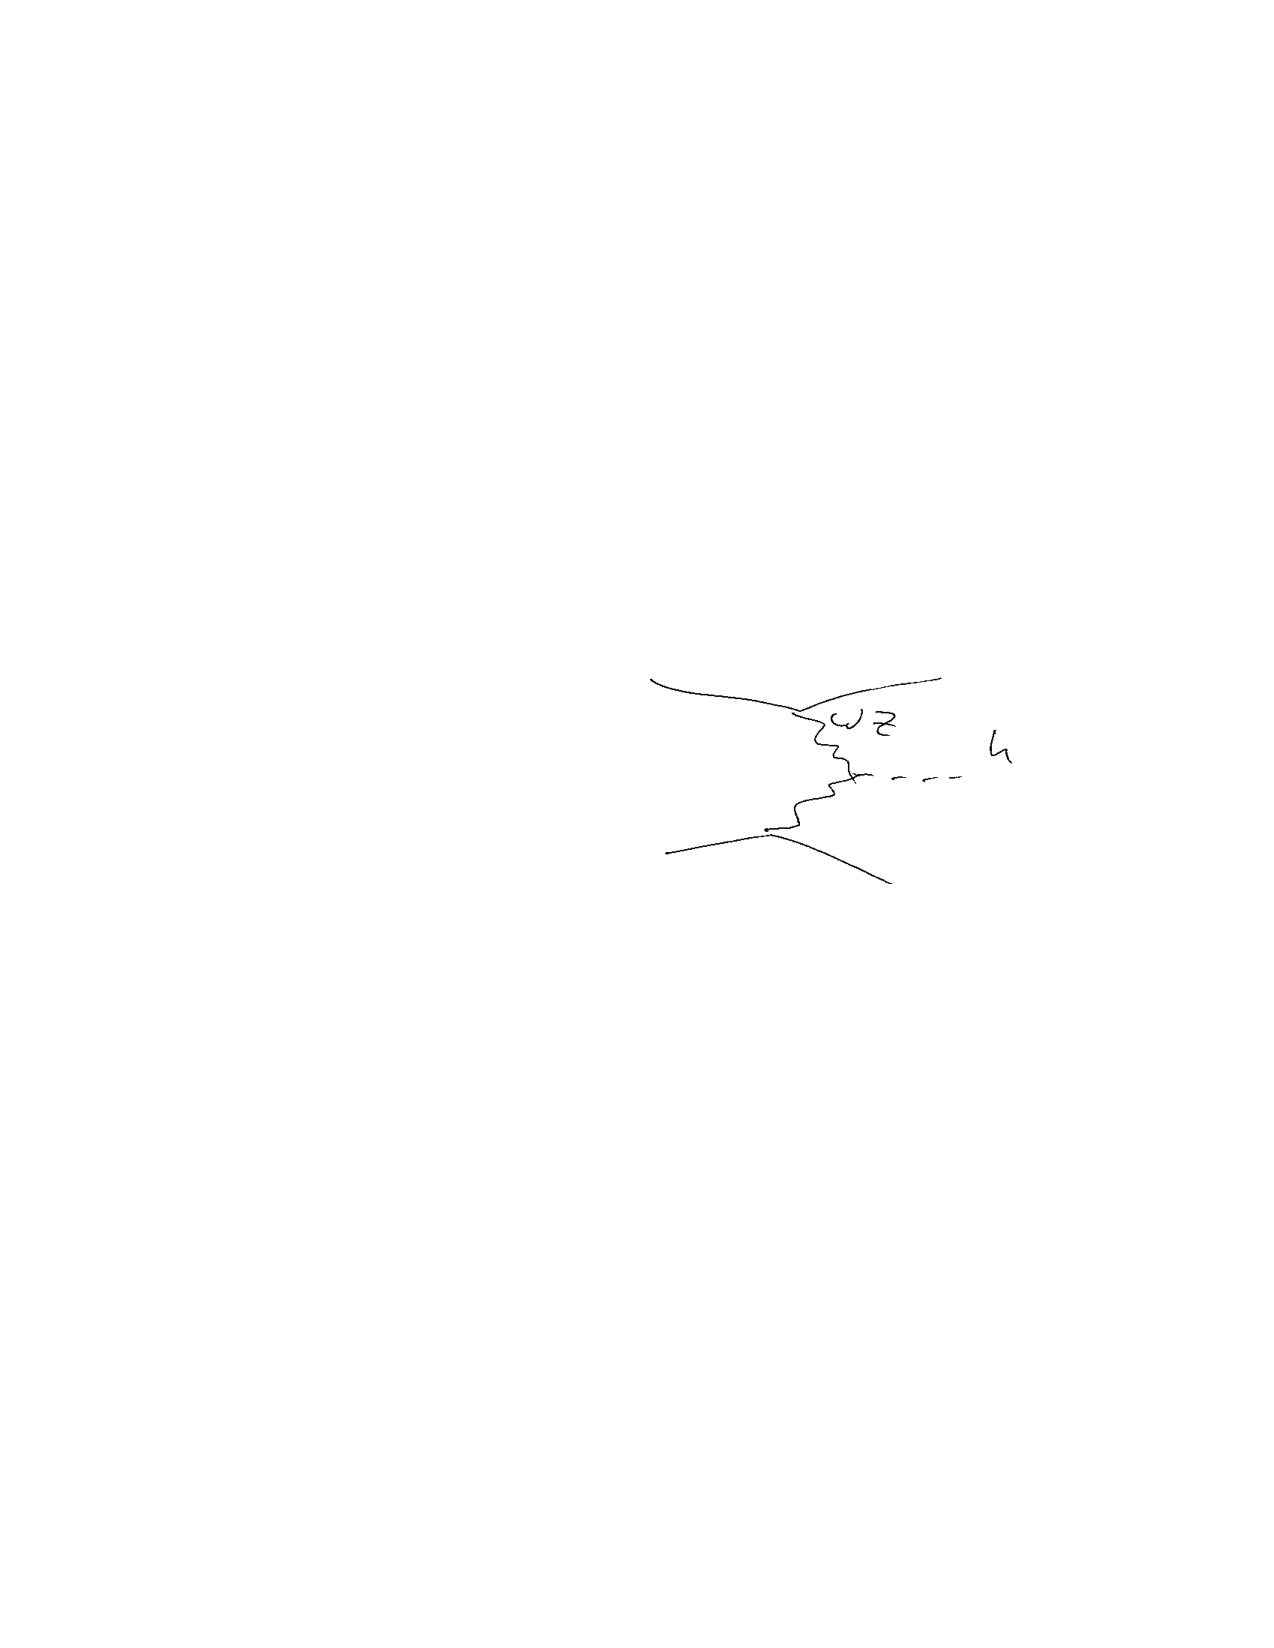
\includegraphics[width=0.4\textwidth]{./VBF.pdf}}_{\rmt{\huge ``Vector Boson Fusion''}}
\ee
This is one reason the Higgs was so hard to find. 
The leading production diagram are from higher order processes.\\
(``god particle'' vs ``god-damned particle'' )

\lineacross 

How much data is needed?

Lets estimate how often we make a Higgs.

\underline{Warm-up} How often do we make a W/Z? 

\bea
\sigma_{W/Z} \sim \frac{\alpha_W}{m_{W/Z}^2} &\sim& \frac{1}{50}\frac{1}{100^2}\ \GeV^{-2}\\
&\sim& 10^{-6}\ \GeV^{-2}
\eea

\be
\sigma_{pp} \sim \GeV^{-2} \Rightarrow 1 W/Z\ \rmt{for every 1 Million pp collisions} 
\ee

\clearpage

\underline{Now lets do the same thing for the Higgs}
\bc
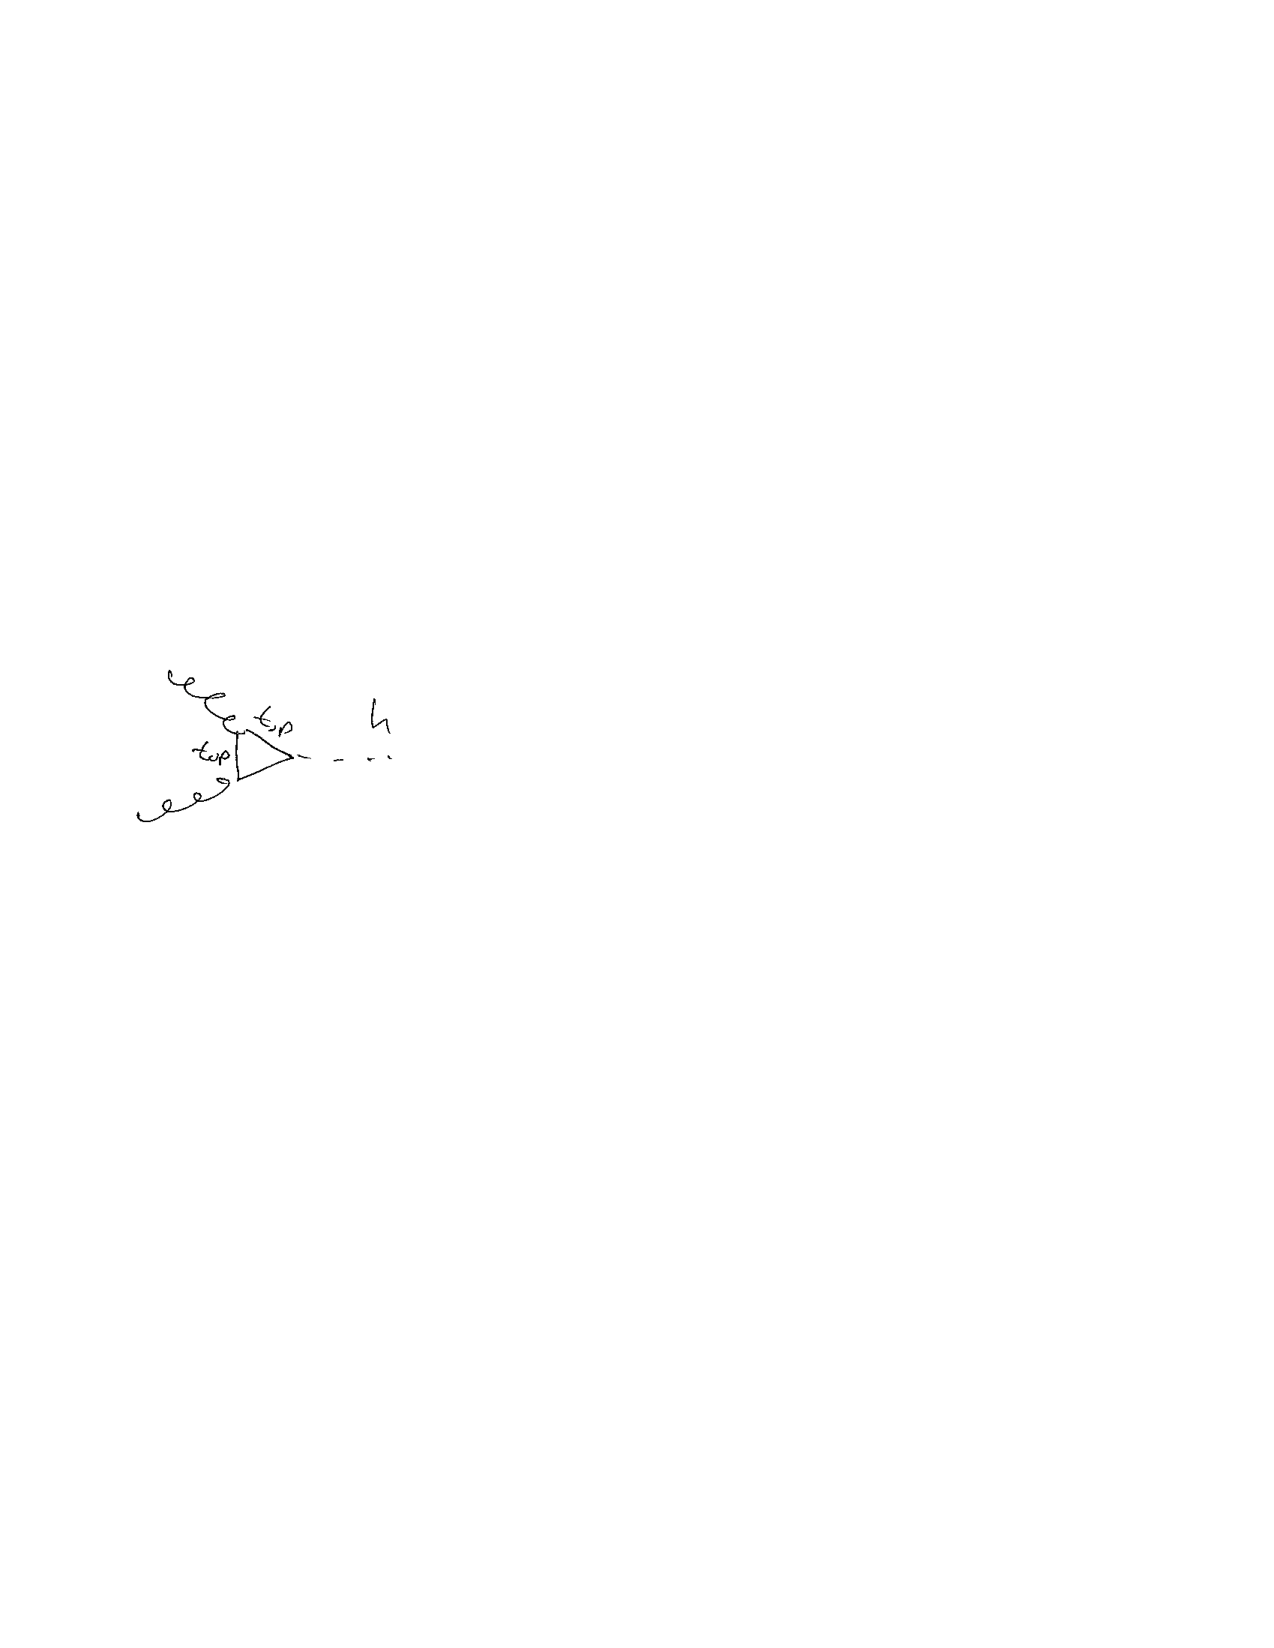
\includegraphics[width=0.4\textwidth]{./ggF.pdf}
\ec
\bea
\sigma_H &\sim& \frac{1}{16\pi^2} \frac{\alpha_s^2 \alpha_W}{m_H^2}\\
&\sim& \frac{1}{160} \left(\frac{1}{10}\right)^2 \left(\frac{1}{50}\right) \left(\frac{1}{100}\right)^2 \GeV^{-2} \sim 10^{-10} \GeV^{-2}
\eea

1 Higgs for every billion proton collisions.

\lineacross
\bc
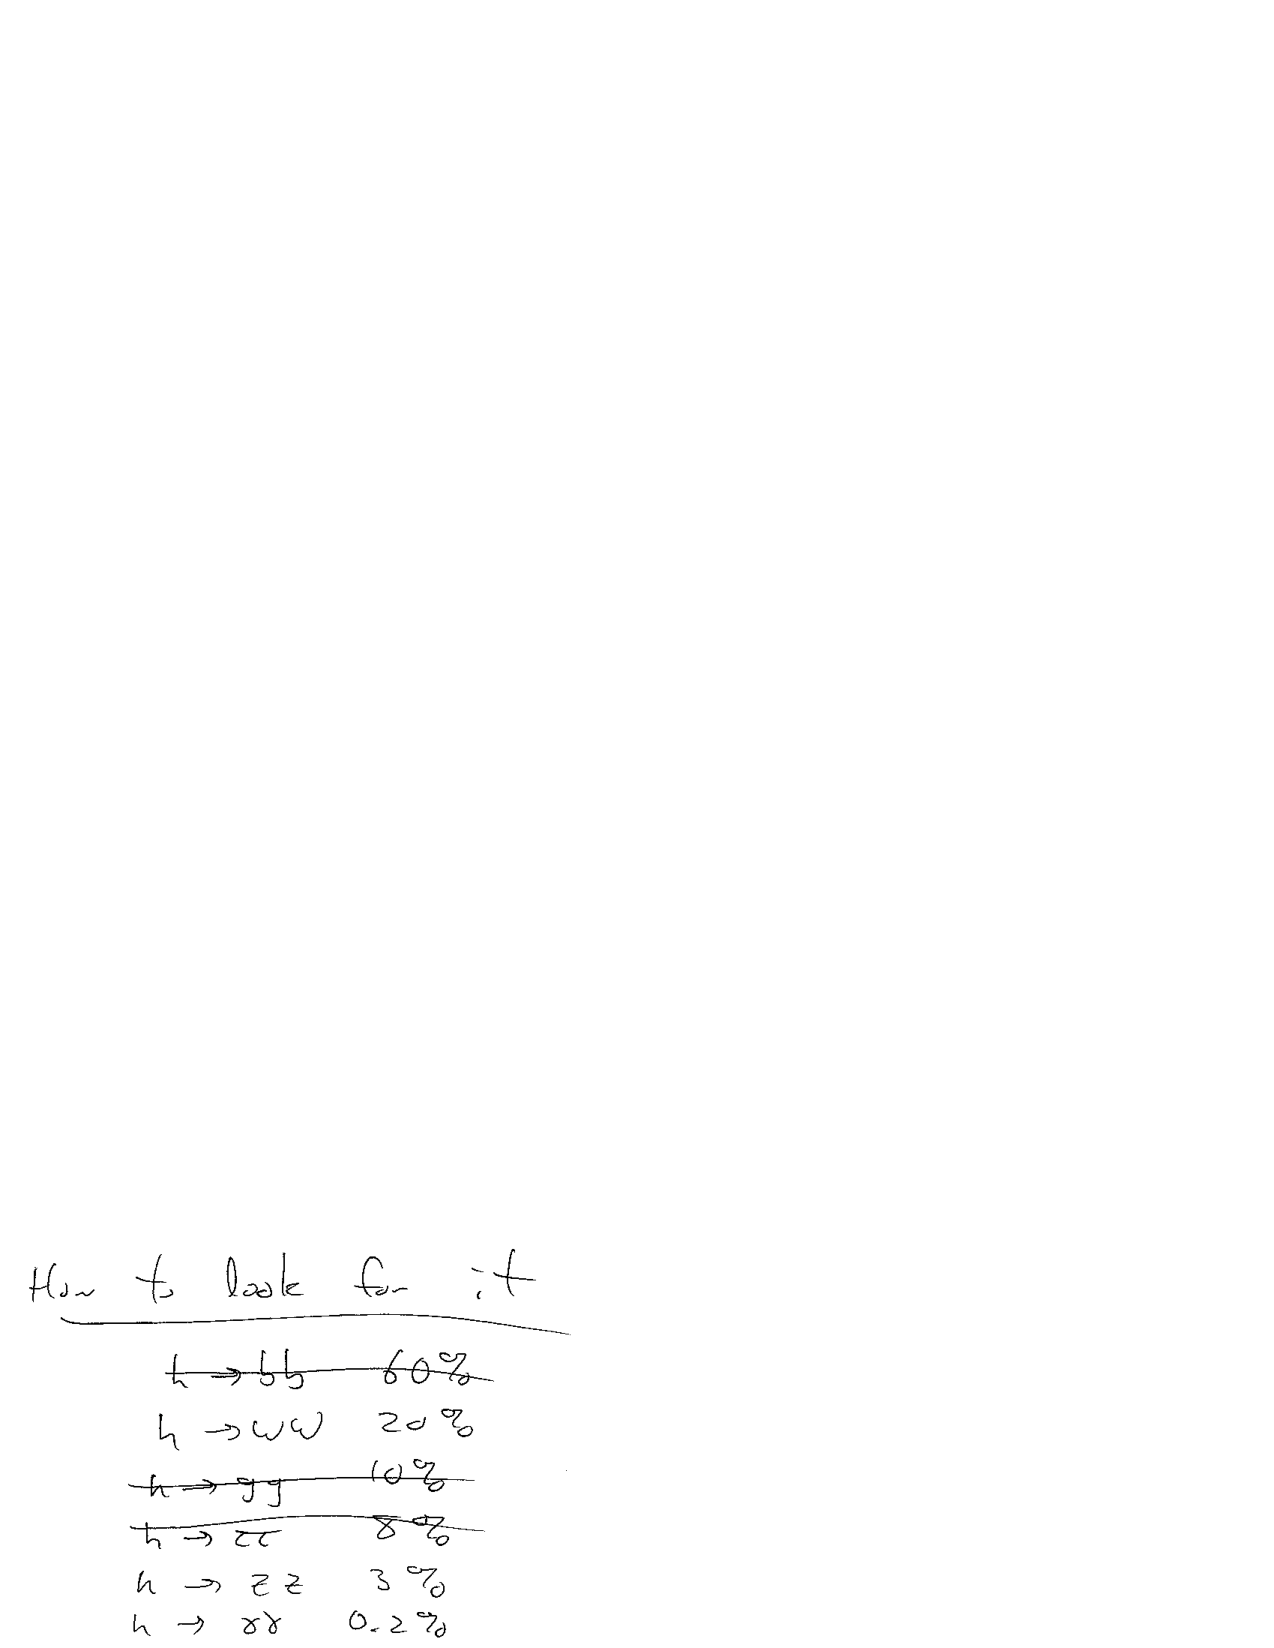
\includegraphics[width=0.5\textwidth]{./HiggsTable.pdf}
\ec

Good target is $\sim$ 100 $\frac{h\rightarrow\gamma \gamma}{\rmt{year}}$

$\Rightarrow 10^5 \frac{\rmt{higgs}}{\rmt{year}} \sim 1 \frac{\rmt{higgs}}{s}$ 

$\Rightarrow$ Need a billion proton collisions per second.

\clearpage

Only have beams that cross at 40 millsion times/s\\
 $\Rightarrow$ need at least 25 proton collisions per crossing. 

This is why we have to live with pile-up. 

In 2012, Higgs discovered 
\bi
\item[-]$ h\rightarrow WW \rightarrow \ell \nu \ell \nu$ (Hard)
\item[-]$ h\rightarrow ZZ \rightarrow \ell \ell \ell \ell$  (easy)
\item[-]$ h\rightarrow \gamma\gamma$  (straight forward)
\ei

\textbf{\underline{Triumph of Humanity!!!}}

Cartoon:
\bc
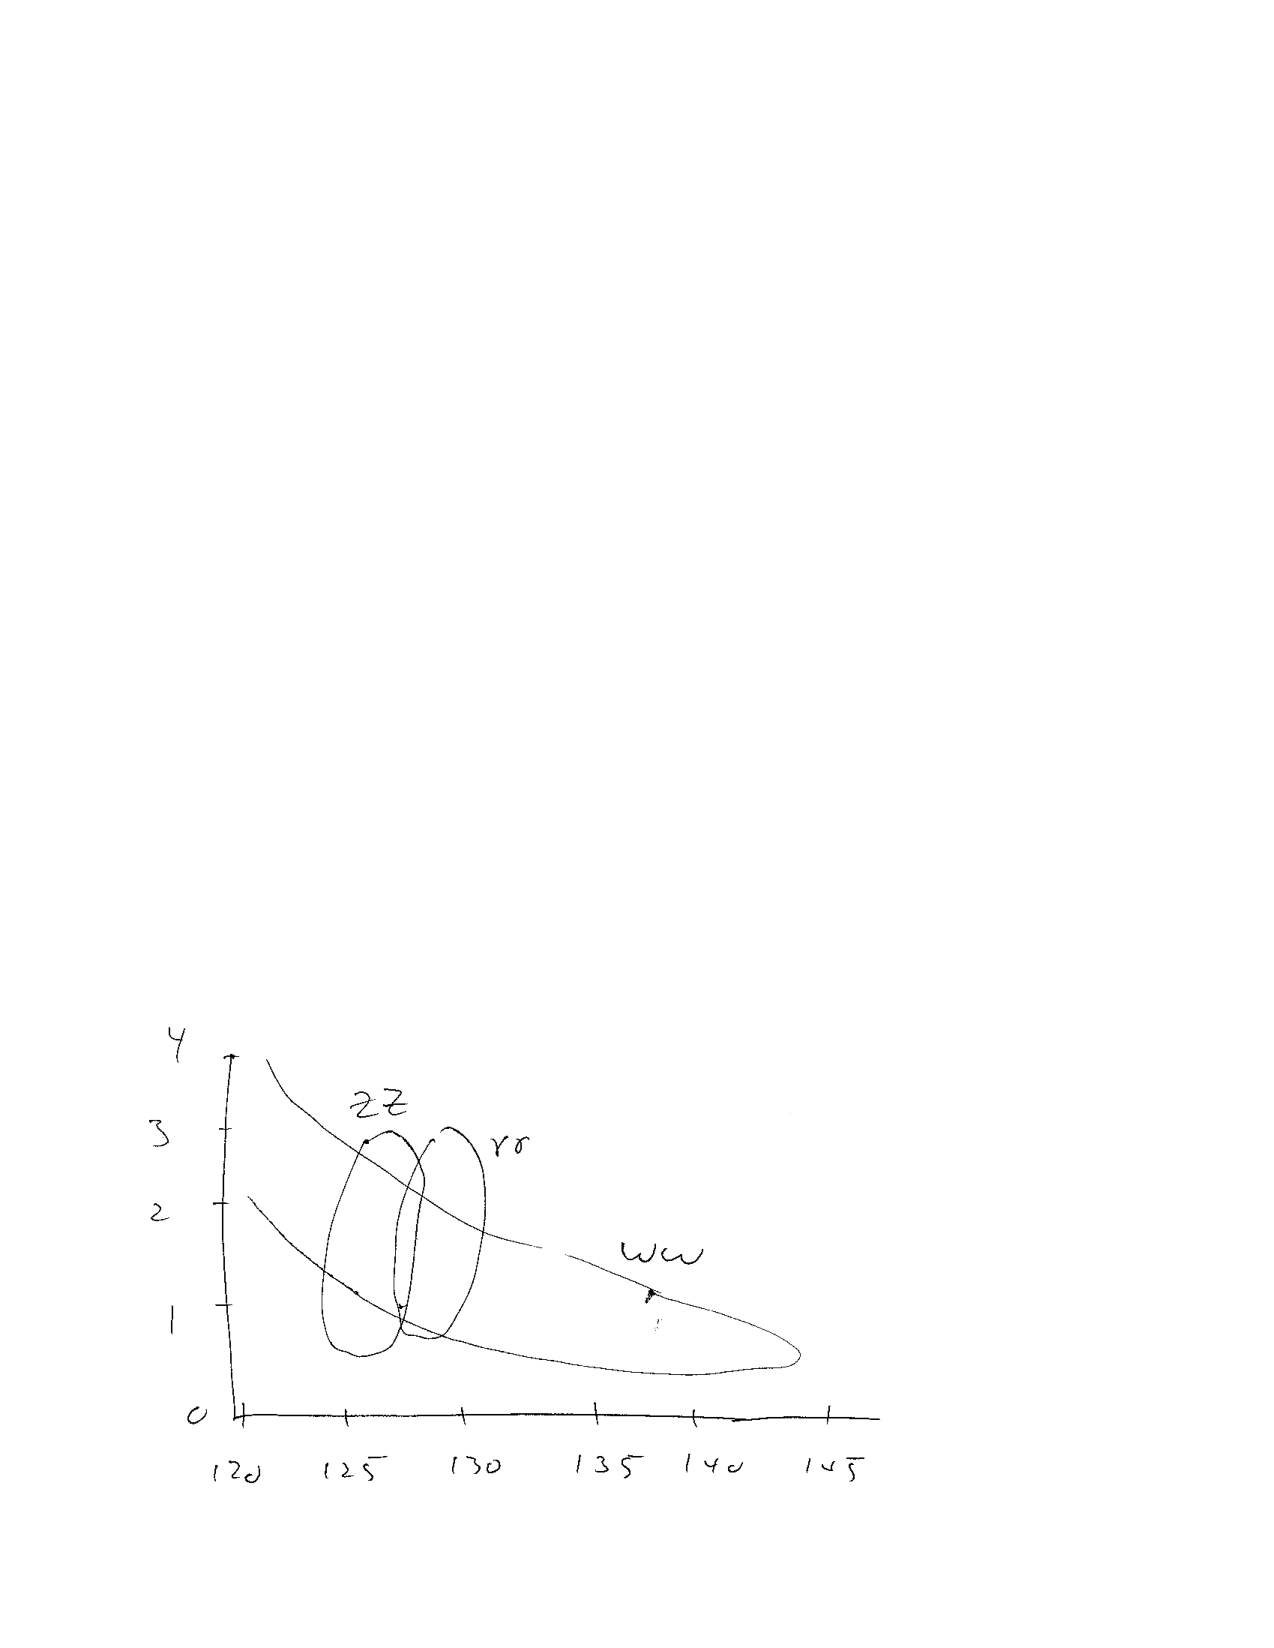
\includegraphics[width=0.5\textwidth]{./HiggsDiscovery2.pdf}
\ec
Real Data:
\bc
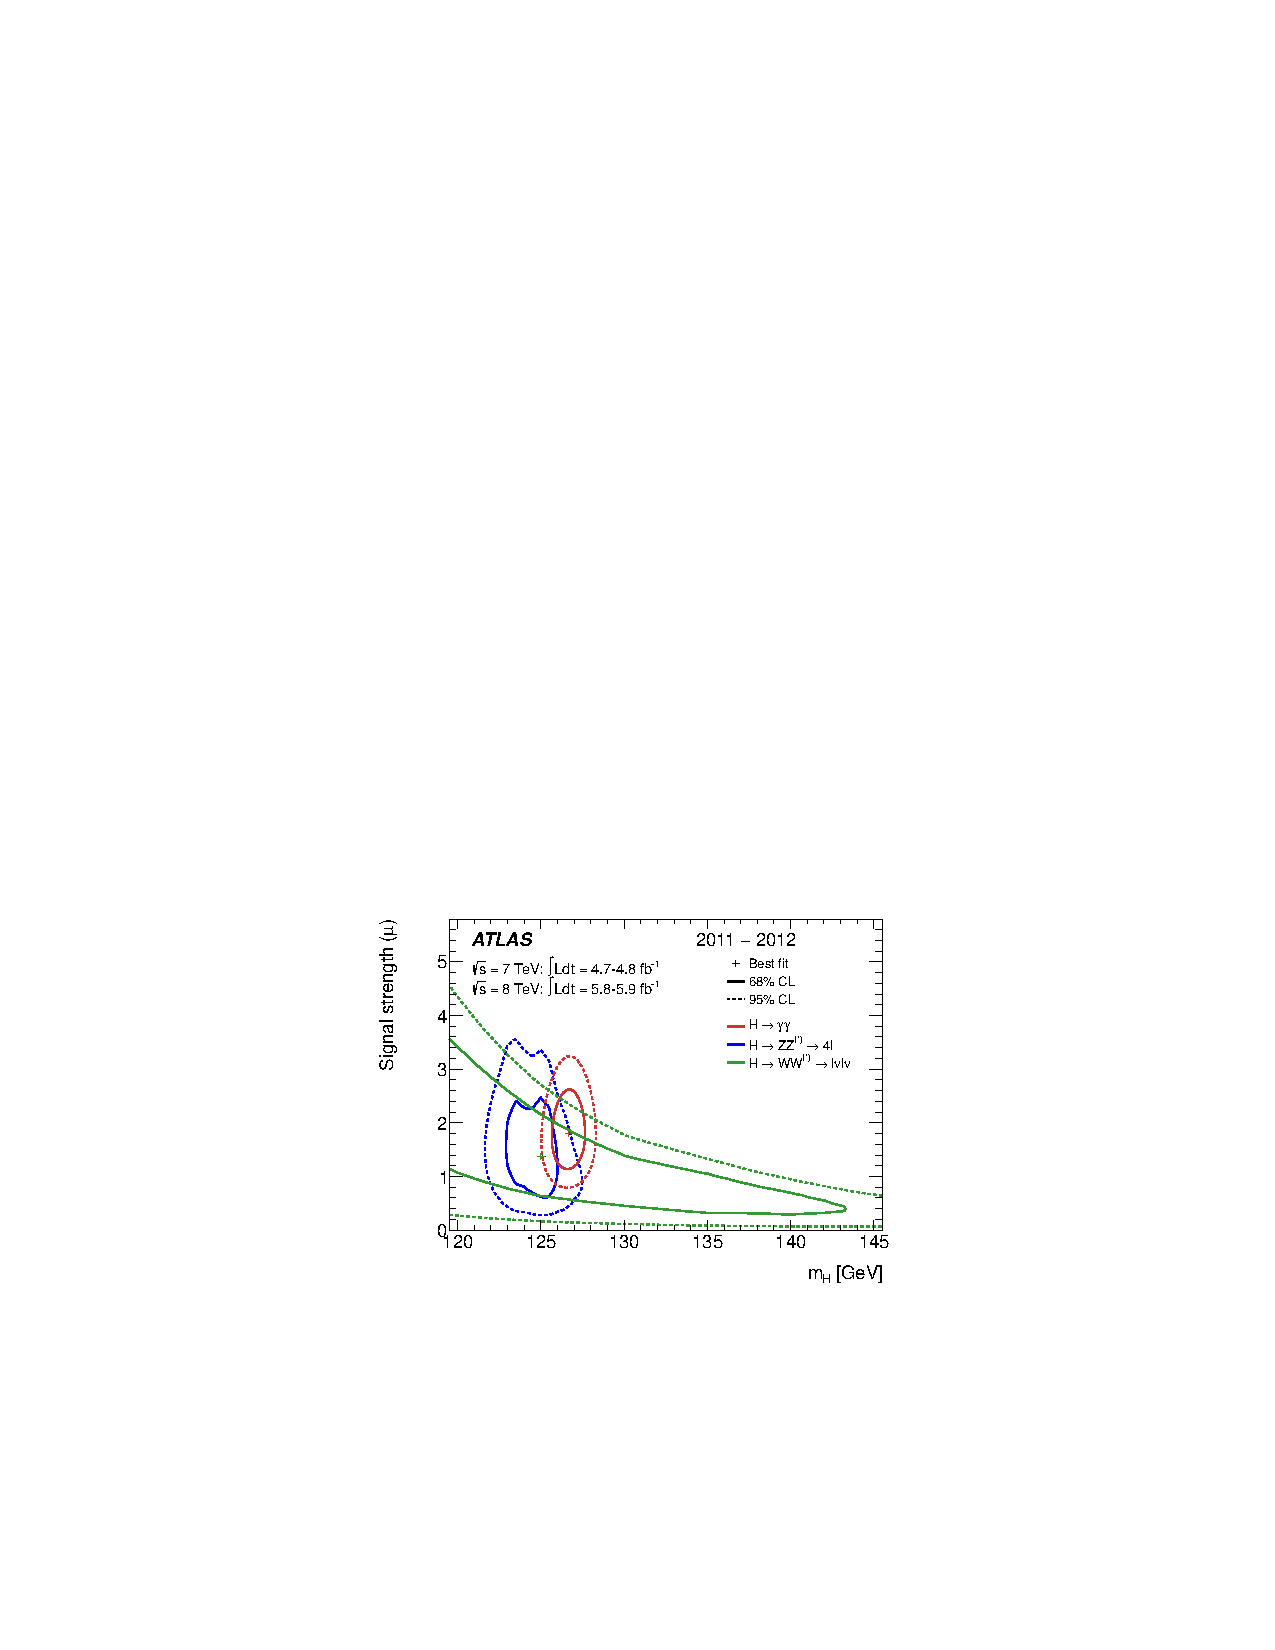
\includegraphics[width=0.5\textwidth]{./BannaPlot.pdf}
\ec

\clearpage

So far looks like SM Higgs in every way.  (stupidest version)

\underline{What we dont know}
\bi
\item[-] if established couoplings are modified at the $\sim 10-20$\% level
\item[-] ${ }$\\ 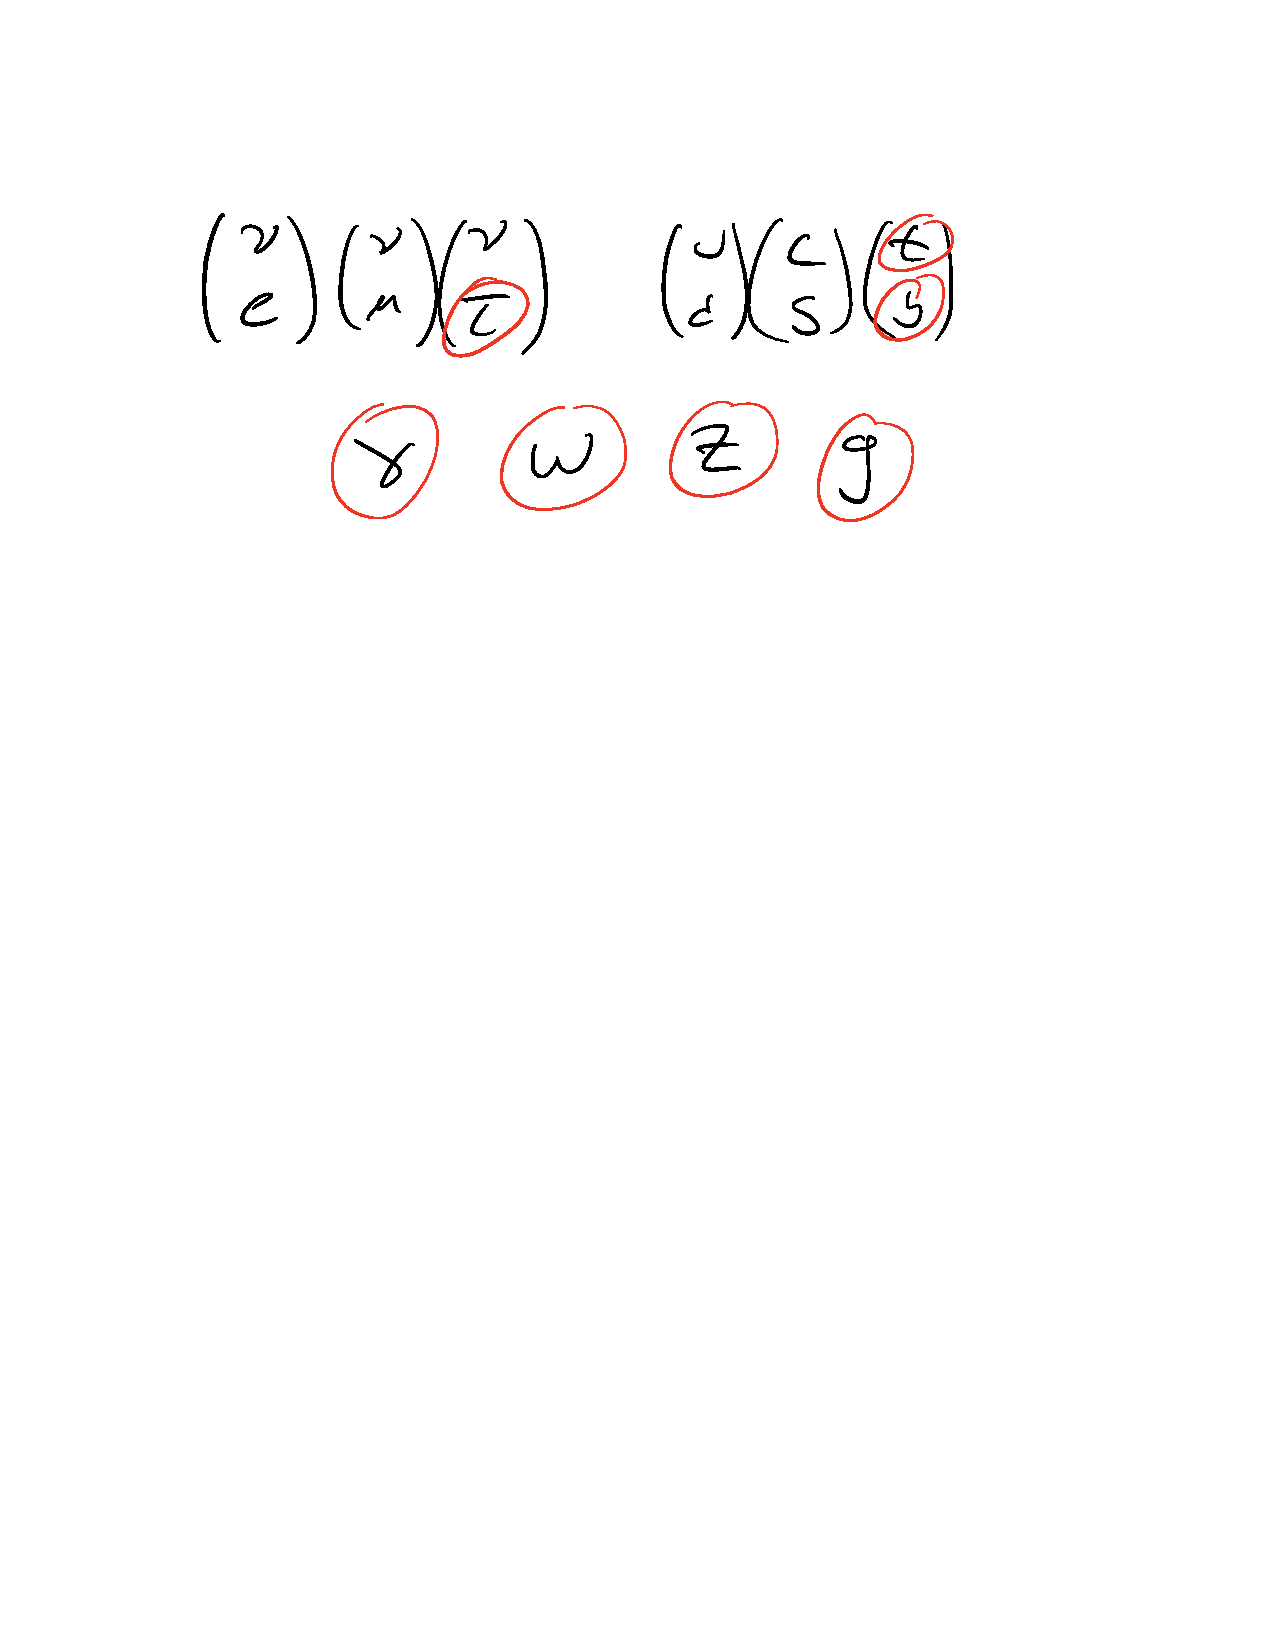
\includegraphics[width=0.5\textwidth]{./SMCouplings.pdf}
\item[-] if Higgs decays in unexpected way $\sim 20$\% of the time
\item[-]{ \underline{Very} important unobserved interaction\\
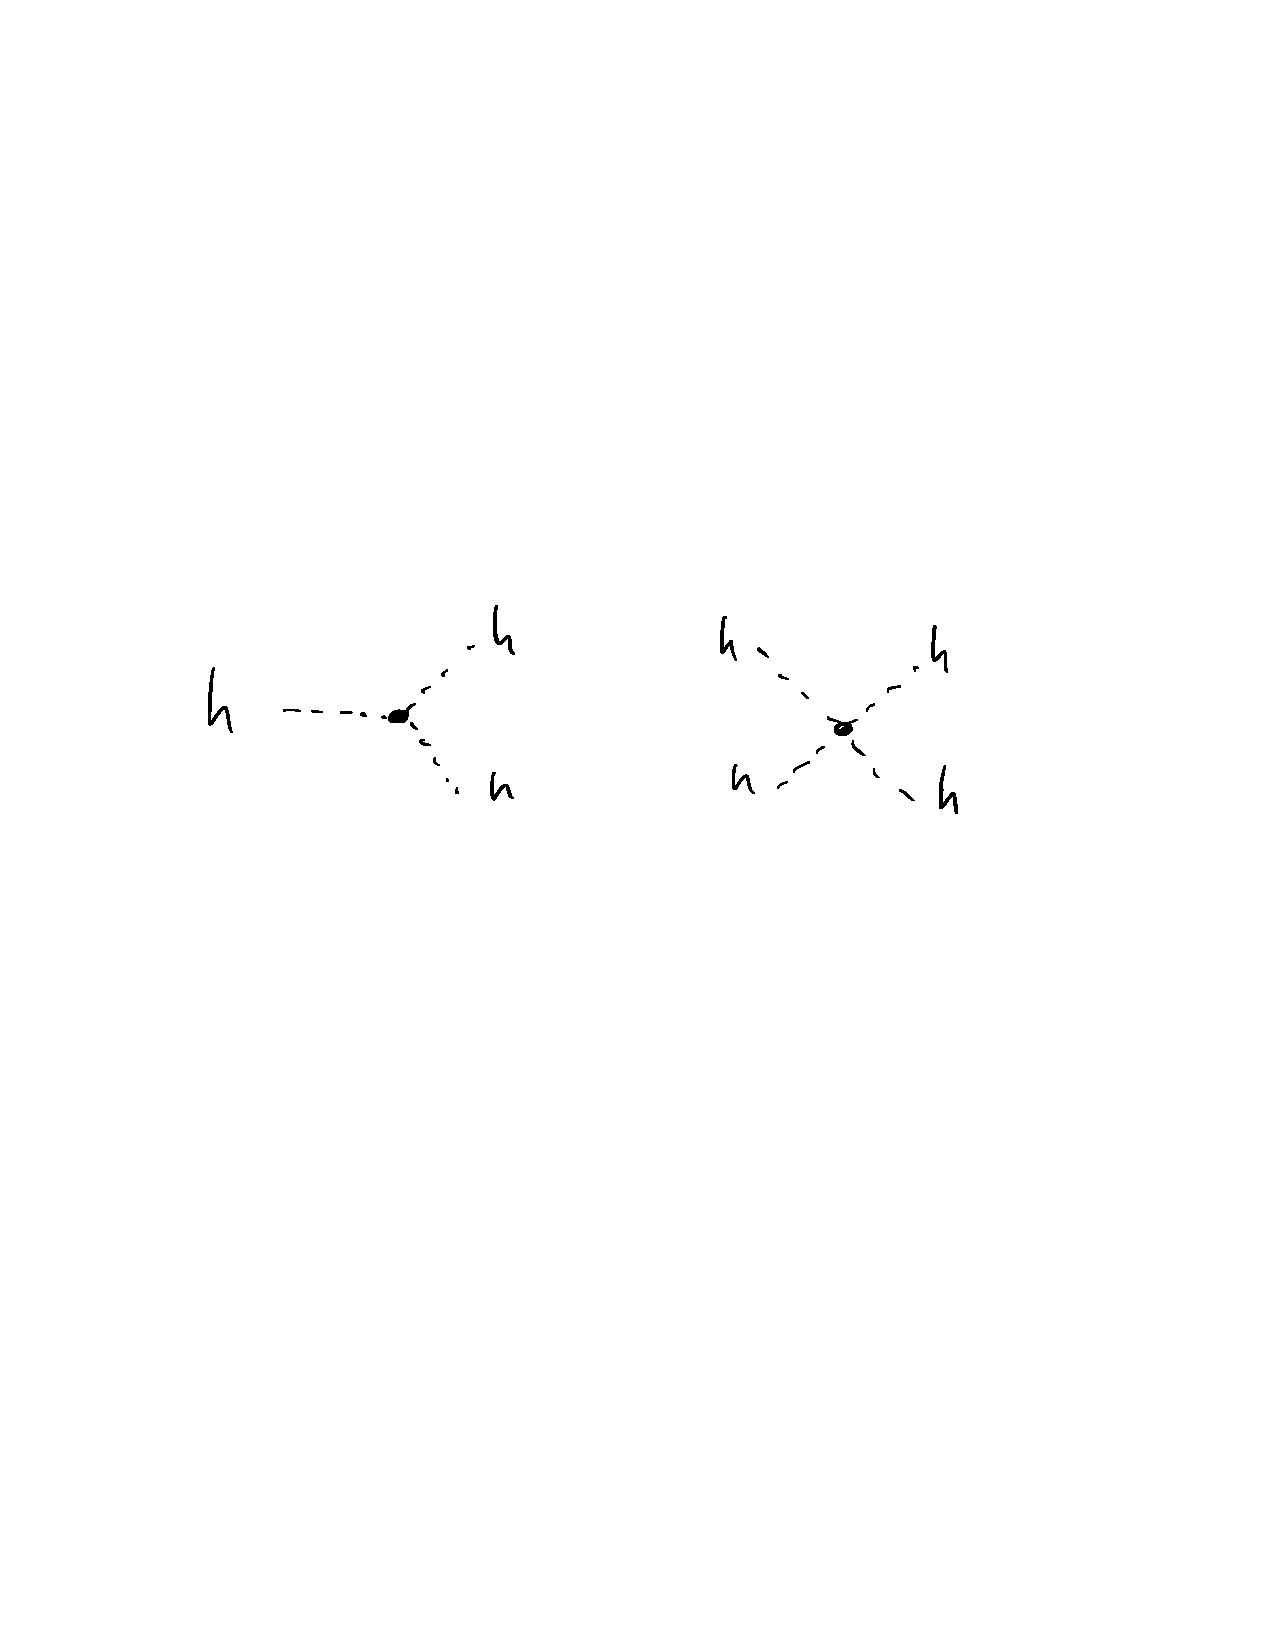
\includegraphics[width=0.7\textwidth]{./HIggsCouplings.pdf}
}
\ei

Higgs self-interaction. 

Di-Higgs Production / Next Frontier.

}
\end{document}


